\documentclass[a4paper,11pt]{article}
\usepackage[left=3cm,top=3cm,right=2cm,bottom=2cm]{geometry}
\usepackage[brazilian, english]{babel}
\usepackage[T1]{fontenc}
\usepackage[utf8]{inputenc}
\usepackage[numbers]{natbib}
\usepackage{epigraph}
\usepackage{indentfirst}
\usepackage{listings}
\usepackage{graphicx}
\usepackage{wrapfig}
\usepackage{setspace}
\usepackage{tablefootnote}
\usepackage[hidelinks]{hyperref}
\usepackage[bottom]{footmisc}
%\usepackage{xcolor}
\usepackage[dvipsnames]{xcolor}
\usepackage{adjustbox}
\usepackage{verbatim}
\usepackage{amsmath}
\usepackage{float}
\usepackage{lmodern}% http://ctan.org/pkg/lm
\usepackage{svg}
\usepackage{xcolor}
\usepackage{array} % for custom space in table columns
\usepackage{makecell}
\usepackage{enumitem}
\usepackage{amssymb}% http://ctan.org/pkg/amssymb
\usepackage{pifont}% http://ctan.org/pkg/pifont
\usepackage{import}
\usepackage{tikz}

% custom link style
\newcommand{\link}[2]{{\color{blue}\underline{\href{#1}{#2}}}}
\newcommand{\tabitem}{~~\llap{\textbullet{\ensuremath{\bullet}}}~~}
\newcommand*{\SignatureAndDate}[4]{%
	\parbox{7cm}{
      \centering
      \rule{6cm}{1pt}
       #1

       #2
    }
    \hfill
\parbox{7cm}{
      \centering
      \rule{6cm}{1pt}
       #3

       #4
    }
}%

% check and uncheck marks for comparison table
\newcommand{\cmark}{\ding{51}}
\newcommand{\xmark}{\ding{55}}

\floatstyle{ruled}
\newfloat{program}{thp}{lop}
\floatname{program}{Program}

\onehalfspacing
\setlength{\parskip}{1em}

% table configuration
\setlength{\tabcolsep}{18pt}
\renewcommand{\arraystretch}{1.5}

\title{Relatório de Estágio III}

\renewcommand{\familydefault}{\sfdefault}

% listing label configuration
\renewcommand{\lstlistingname}{Código}
\renewcommand{\lstlistlistingname}{Lista de \lstlistingname s-Fonte}

% additional libraries for tikz
\usetikzlibrary{trees,positioning,shapes,shadows,arrows}

% command to center column labels when column is left aligned
\newcommand*{\centerhead}[1]{\multicolumn{1}{|c|}{#1}}

\begin{document}
\selectlanguage{brazilian}

%%% CAPA %%%

\begin{titlepage}

\begin{wrapfigure}[2]{l}{0.2\textwidth}
	\label{Logo UFABC}
	\vspace{-1\baselineskip}
	\centering
	
\includegraphics[width=0.25\textwidth]{images/Logo_UFABC}
\end{wrapfigure}

\uppercase{Universidade Federal do ABC}

\uppercase{Bacharelado em Ciência da Computação}

\vfill
\begin{center}

\uppercase{\textbf{Projeto de Graduação em Computação}}

\vfill

\uppercase{Bruno Cesar Porto de Arruda}
\vspace{1cm}

Orientador: Prof. Dr. Vladimir Moreira Rocha

\vfill

Santo André -- SP

2019
\end{center}
\end{titlepage}

%%% FIM DA CAPA %%%

%%% FOLHA DE ROSTO %%%

\begin{titlepage}
\begin{center}
\uppercase{\textbf{Bruno Cesar Porto de Arruda}}

\vfill

\uppercase{\textbf{SmartDCPABE: Um sistema distribuído com permissão de acesso a prontuários de pacientes por meio de Smart Contracts}}
\end{center}

\vfill

\hfill \begin{minipage}{0.5\textwidth}
Trabalho submetido à Universidade Federal do ABC como parte dos requisitos para a conclusão do Bacharelado em Ciência da Computação.
\vspace{1cm}

Orientador: Prof. Dr. Vladimir Moreira Rocha
\end{minipage}

\vfill

\begin{center}
Santo André -- SP

2019
\end{center}
\end{titlepage}

%%% FIM DA FOLHA DE ROSTO %%%

\begin{center}
\uppercase{\textbf{Dedicatória}}
\end{center}
	xxx.


\newpage
\begin{center}
\uppercase{\textbf{Agradecimentos}}
\end{center}

\noindent	Ofereço meus sinceros agradecimentos:

\vspace{1cm}


%%% ABSTRACT - PORTUGUÊS %%%
\newpage
\begin{abstract}

\noindent Blockchain é uma tecnologia inovadora para o compartilhamento de informações entre organizações de maneira descentralizada sem a necessidade de depender de uma autoridade central.
Na área da saúde, o compartilhamento de dados médicos permite a melhoria na qualidade do atendimento e a redução de custos de operação, entretanto, obstáculos técnicos tem impedido a comunicação dos sistemas de saúde, envolvendo questões como privacidade, segurança, integridade e interoperabilidade destes sistemas.
Atualmente quem define as condições de acesso aos dados médicos é a instituição que fez seu registro, quando na verdade deveria ser o próprio paciente, uma vez que o prontuário médico é do paciente por direito.
Além do paciente não poder controlar ou consentir sobre o acesso ao prontuário, ele próprio não possui este acesso, que é cedido mediante requerimento.
Neste trabalho, propomos um sistema distribuído baseado em Blockchain para o compartilhamento e controle de acesso a prontuários médicos.
O controle é centrado no paciente, que pode definir políticas de acesso usando criptografia baseada em atributos (CBA) gerados pelas instituições que atuam como certificadoras no sistema.
Usuários e instituições interagem entre si por meio de Smart Contracts na rede Ethereum e também os utilizam para consulta de metadados de arquivos e atributos publicados por certificadores.
Analisamos os limites de compatibilidade na codificação das estruturas de dados da CBA em uma transação Ethereum e implementamos um protótipo para verificar a viabilidade da implantação e operação do sistema em termos de consumo de gas.

\noindent \textbf{Palavras-Chave:} Blockchain; Ethereum; Contratos Inteligentes; CBA; DCPABE; RES.
\end{abstract}

%%% ABSTRACT - INGLÊS %%%

\newpage
\selectlanguage{english}
\begin{abstract}
\noindent Blockchain is an innovative technology to share data among institutions in a decentralized and trustless way, without the need of relying on a central authority.
In Healthcare sector, data sharing improves the quality of medical care and reduce operation costs, but technical problems have hindered the communication of health systems, problems such as privacy, security, integrity and interoperability.
Nowadays, the institution who produced the medical data usually is the one that control the access of that data, when in fact the control should be exercised by the patient, the owner of such data.
Besides the patient cannot control ou consent upon the access conditions to his personal data, he evens has access to it, which is made available only upon request.
In this work, we propose a distributed, Blockchain-based system for sharing and access control of Health Recordings.
The control is patient centric as he is responsible for the access policies described in terms of attributes generated by institutions that plays the role of authorities in a attribute-based Cryptography (ABE) scheme.
Users and institutions use Smart Contracts on a Ethereum network to interact and query about record metadata and attributes published by certifiers.
We analyse the compatibility limits in the codification of ABE data structures in a Ethereum transaction and we implement a prototype to verify the viability of system implantation and operation, in terms of gas consumption.

\noindent \textbf{Keywords:} Blockchain; Ethereum; Smart Contracts; ABE; DCPABE; EHR.
\end{abstract}

\selectlanguage{brazilian}

%%% SUMÁRIO %%%
\newpage
\tableofcontents

%%% LISTA DE CÓDIGOS %%%
\newpage
\lstlistoflistings

%%% LISTA DE FIGURAS %%%
\newpage
\listoffigures

%%% LISTA DE TABELAS %%%

\newpage
\listoftables

% -------------------------------------------------------------------- %
\newpage
\section{Introdução}

{\color{blue} A tecnologia Blockchain~\cite{nakamoto2008bitcoin} permite o armazenamento confiável e distribuído das informações ...}

A tecnologia Blockchain permite o armazenamento confiável e distribuído de informações, sem a necessidade de uma autoridade confiável central \cite{Swan2015}.
A principal inovação da Blockchain foi eliminar a necessidade de uma contraparte confiável e distribuir a manutenção da rede aos próprios integrantes, que tem suas atividades coordenadas por uma nova gama de algoritmos de consenso.
Essa família de algoritmos de consenso apresentam duas diferenças fundamentais em relação aos modelos tradicionais descritos na literatura quanto às premissas envolvidas \cite{Narayanan2016a}.
A primeira diferença é a ideia do incentivo, introduzida no consenso da Blockchain ao exigir o consumo de recursos computacionais para participação na rede e ao alinhar a possibilidade de ganho ao comportamento honesto e de prejuízo à tentativa de corromper ou alterar os registros da rede.
A segunda diferença é a noção estatística do consenso, isto é, enquanto algoritmos de consenso tradicionais modelam soluções que eventualmente encerram seu processamento e retornam uma decisão unânime e irrevogável, o protocolo da rede Bitcoin é fundamentalmente estocástico e contínuo ao longo do tempo.
Para exemplificar, em termos práticos estima-se que o consenso sobre a validade de uma transação no Bitcoin leve em torno de uma hora, porém, mesmo após este tempo, não é possível ter certeza absoluta sobre a validade desta transação.
De fato, o que ocorre é que a chance de reversão da transação (isto é, alteração do consenso estabelecido na rede para um estado onde a transação seja inválida) cai exponencialmente com o passar do tempo e o processamento de novas transações.

{\color{blue} Inicialmente, ela foi usada no contexto de transações financeiras, mas foi expandida e tem sido utilizada em diversos outros contextos, sendo na área de saúde um deles ...}

A ideia dos incentivos no consenso da Blockchain foi inicialmente usada no contexto de transações financeiras por meio do Bitcoin \cite{nakamoto2008bitcoin} e seu sucesso incentivou a proposta de novos protocolos de Blockchain e de mecanismos de consenso para diversos outros contextos, onde ocorre a troca e criação de qualquer tipo de ativo, financeiro ou não-financeiro.
A vantagem de permitir a interação segura e confiável entre duas partes sem arcar com os custos de transação de uma terceira parte abre caminho para a formação de consórcios entre empresas de diversos segmentos onde a troca de informações agregue valor ao produto ou serviço \cite{Wust2017}.
Um exemplo de área que se beneficia de tal integração é a área da saúde, uma vez que a qualidade do serviço prestado ao paciente aumenta se houver disponibilidade de seu histórico médico, que está distribuído pelas instituições que o atenderam no curso de vida dele.

{\color{blue} A expansão foi possível pela inserção de contratos inteligentes, softwares que possibilitam a inserção de regras de negócios na Blockchain}

Inicialmente, novas soluções baseadas em Blockchains lançavam sua própria rede, personalizando transações e regras de validação para atender a área de aplicação do projeto.
Uma nova abordagem para soluções em Blockchain surgiu com a Ethereum \cite{Buterin2014}, uma Blockchain capaz de emular uma máquina virtual distribuída, na qual é possível implantar e interagir com Smart Contracts.
Smart Contracts são programas que reagem à interação de um usuário ou de outro contrato, com capacidade para possuir estruturas de dados e regras de negócio arbitrárias.
Os Smart Contracts se tornam interfaces de consulta e de alteração do estado da Blockchain, facilitando o desenvolvimento de novas soluções distribuídas (denominados como \emph{dApps}) sem as complicações de desenvolvimento e de risco de segurança de implantar uma rede própria.

{\color{blue} Na área de saúde, os trabalhos propõem armazenar os prontuários dos pacientes na Blockchain...}

{\color{blue} Entretanto, os prontuários não podem ser armazenados diretamente por duas razões: (1) problema de espaço no armazenamento ... (2) problema de visibilidade de dados sensíveis ...}

Soluções baseadas em Blockchain com suporte nativo a Smart Contracts como a Ethereum possuem um problema relacionado ao armazenamento, por basicamente dois fatores.
Primeiro, existe um custo associado ao uso, o que torna inviável o armazenamento de dados muito extensos.
Mesmo que exista uma amplitude de recursos para se despender no uso da Blockchain, há uma limitação imposta ao tamanho de uma transação e, consequentemente, no volume de dados que pode ser publicado por meio dela.
Segundo, dados na Blockchain são inerentemente visíveis a todos os usuários, inviabilizando o seu uso para o armazenamento de informações sensíveis.
Mesmo informações criptografadas correm risco se forem incluídas na Blockchain, uma vez que não é possível nem apagar ou alterar a senha usada na geração do conteúdo criptografado, pondo em risco o sigilo da informação em caso de vazamento de senha.

{\color{blue} Nesse sentido, este trabalho propõe um sistema, baseado em contratos inteligentes, que permite o acesso aos prontuários. Para isso, foi criado um modelo de dados específico para lidar com o espaço de armazenamento e foi usada a encriptação baseada em atributos para lidar com o problema da visibilidade de dados ...}

Este trabalho apresenta um sistema distribuído de compartilhamento de arquivos médicos por meio de Smart Contracts que registram informações sobre arquivos médicos, que são armazenados fora da Blockchain e tem seu conteúdo protegido contra o acesso não autorizado por meio da criptografia baseada em atributos.
Este trabalho também propõe uma taxonomia para fundamentar a criação de atributos para uso na criptografia a deriva algumas políticas de acesso em termos destes atributos que podem vir a ser utilizadas em cenários de uso reais, modelados a partir da análise das regras na legislação
brasileira que disciplinam as condições de acesso ao prontuário de um paciente .

\subsection{Objetivo geral}

Criar um sistema distribuído, com base em Smart Contracts executados em uma Blockchain, que permita o acesso a prontuários eletrônicos dos pacientes por meio de políticas de acesso baseadas em atributos.

\subsection{Objetivos específicos}

\begin{itemize}

\item Criar uma taxonomia de permissões no contexto de saúde.

\item Analisar como funciona a criptografia baseada em atributos (\textit{attribute-based encryption}, em inglês).

\item Analisar como funcionam a tecnologia Blockchain Ethereum e os contratos inteligentes.

\item Implementar os contratos inteligentes para dar acesso aos prontuários eletrônicos utilizando a taxonomia e a criptografia baseada em atributos.

\item Implantar e executar os contratos inteligentes em uma arquitetura Blockchain.

\end{itemize}

\subsection{Justificativa}

% -------------------------------------------------------------------- %
\newpage
\section{Fundamentação Teórica}

\begin{itemize}
    \item {\color{red}Cada parágrafo deve ter em torno de 10 linhas}
    \item {\color{red}Não mostrar código.}
\end{itemize}

\subsection{Criptografia Baseada em Atributos} \label{sec:sub:abe}

{\color{ForestGreen}Explicar quando nasceu, quem a criou, e qual foi o problema que estava resolvendo (basicamente que a criptografia chaves publica/privada precisa ser criada para cada usuário que precisa de permissão e com a por atributos não). (2 parágrafos).} % TODO: (ok) padronizar acesso e permissão, fica confuso usar diferentes palavras para o mesmo conceito. Se forem diferentes, explicar

A criptografia assimétrica pode ser vista como um mecanismo para que um usuário, Alice, codifique dados de forma confidencial e os aderece a um destinatário, Bob.
Para que seja viável criptografar um conteúdo desta forma, geralmente é necessário que exista uma Infraestrutura de Chaves Pública \emph{(Public Key Infrastructure - PKI)} para incluir Bob ao sistema, atribuindo-lhe um par de chaves pública-privada.
Os primeiros métodos de geração de chaves usavam processos aleatórios para produzir a chave privada, que gerava uma chave pública que também se assemelhavam a valores aleatórios para um observador que não possua a chave privada.
Por conta disso o PKI também tem a tarefa de administrar um diretório de certificados, que tipicamente carregam informação da chave pública, seu titular, autoridade emissora e também sua validade.
Se torna necessário consultar este diretório para descobrir quem são os usuários do sistema e mesmo com estas informações sendo armazenadas localmente, ainda será necessário verificar continuamente se as chaves foram revogadas, seja por expiração da data de validade ou por decisão da autoridade outorgante.
A necessidade da consulta e validação de chaves públicas no diretório de certificados restringe a criptografia à disponibilidade de conexão à fonte de consulta.
Ademais, como as chaves públicas não tem relação intrínseca com a identidade de seu representado, não é possível criptografar conteúdos a destinatários que ainda não possuam uma chave, sendo necessário postergar o envio das informações, permanecendo neste meio tempo sem formas de usar o sistema oferecido pela PKI para garantir o sigilo das informações.

Visando eliminar tais restrições, Shamir idealizou em 1984 a Criptografia Baseada em Identidades \emph{(IBE - Identity-Based Cryptography)}, um esquema onde as chaves públicas utilizadas para criptografia seriam as próprias formas textuais de identificação de uma pessoa, tais como e-mail, nome completo, números de documento ou qualquer combinação arbitrária destes dados.
Chaves privadas seriam derivadas adicionando à chave pública um parâmetro fixo e secreto, sob controle de uma terceira parte confiável responsável por gerenciar a requisição, geração e entrega de chaves privadas \cite{Shamir1985}.
Somente anos mais tarde, em 2001, surgiu a primeira proposta efetivamente segura e prática de implementação da IBE, propondo também cenários de uso onde seria possível obter mecanismos de revocação automática de usuários e controle de acesso por meio da adição de marcações com significado nas chaves públicas \cite{Boneh2001}.
Por exemplo, ao criptografar e enviar um arquivo usando identidade de Bob concatenada com ano atual (``\emph{ano-2020}''), pode-se conceber um cenário onde Bob devesse solicitar ao gerador de chaves a chave privada correspondente à chave pública ``\emph{Bob@mail.com ano-2020}'', levando a requisições periódicas de novas chaves em anos subsequentes e implementando uma forma efetiva e automática de revocação de acesso de usuários simplesmente ao deixar de conceder novas chaves.
Adicionando tags do tipo ``\emph{acesso=restrito}'' ao exemplo anterior pode-se compreender um cenário onde o usuário precise concordar previamente com termos de compromisso definidos pela administração do gerador de chaves para então obter a chave privada que corresponda à identidade na forma ``\emph{Bob@mail.com ano-2020 acesso=restrito}'' e finalmente ter acesso ao conteúdo que havia sido criptografado com essa chave pública.

A Criptografia Baseada em Atributos (em inglês, \emph{ABE - Attribute-Based Encryption}) visa aumentar a expressividade da IBE ao modelar identidades como um conjunto de atributos, definir chaves públicas como subconjuntos de atributos e tornar a descriptografia possível ao usuário que possuir as chaves privadas correspondentes a estes atributos \cite{Sahai2005}.
Na ABE, atributos representam grupos de usuários ou funções desempenhadas por eles, permitindo expressar políticas de acesso de forma simples e eficaz sem a necessidade do conhecimento prévio da identidade exata de todas as pessoas que deveriam ter acesso aos dados criptografados.
Indivíduos precisariam se autenticar junto a uma autoridade certificadora para obter as chaves privadas pessoais correspondentes a cada atributo que precisarem para operar no sistema, conseguindo realizar o acesso dos dados cujas políticas de acesso consigam satisfazer com os atributos em sua posse.
Para impedir ataques de conluio \emph{(collusion attacks)}, onde um usuário com atributos ``$A$'' e ``$B$'' e outro com atributos ``$C$'' e ``$D$'' unam suas chaves privadas para satisfazer uma política de acesso que exija ``$A \wedge D$'', se faz necessário que a chave privada pessoal relacionada a um atributo seja diferente a cada emissão e preferencialmente que seja atrelada a alguma característica exclusiva do usuário, como número de identidade ou leitura biométrica \footnote{Subsequente ao trabalho de Sahai e Waters, um trabalho de Juels e Szydlo propôs outra noção para ABE, onde não haveria resistência contra ataques de colusão. Para mais detalhes, ver \cite{Juels2004}.}.

{\color{ForestGreen}Explicar alguns conceitos da CBA (chave pública/privada/etc para que sirva como base do exemplo mostrado no último parágrafo (1 parágrafo).}

As políticas de acesso usadas na ABE são traduzidas em um Esquema de Compartilhamento de Segredo (em inglês, \emph{SSS - Secret Sharing Scheme}), onde os atributos ocupam o papel de participantes do esquema e o segredo a ser reconstruído pelo SSS é parte necessária para a execução do algoritmo de descriptografia.
Um esquema de compartilhamento também implica em alguma estrutura de acesso que defina todos os subconjuntos válidos de participantes que deveriam ser capazes de reconstruir o segredo com suas partes.
Shamir demonstrou como produzir estruturas de acesso com uma porta de limiar $(k,n)$, permitindo a reconstrução do segredo se $k$ entre os $n$ participantes se unirem e impedindo, para números menores do que $k$, a reconstrução ou qualquer ganho de informações quanto ao segredo \cite{Shamir1979}.
Benaloh expandiu a ideia, descrevendo esquemas eficientes para estruturas de acesso que pudessem ser descritas em termos de fórmulas monótonas, isto é, fórmulas booleanas utilizando operadores lógicos binários $AND$ e $OR$ e os participantes como predicados \cite{Benaloh1988}.
Desta forma a ABE consegue descrever políticas de acesso como fórmulas booleanas e computar de forma eficiente se os atributos apresentados formam um dos subconjuntos de atributos definidos como válidos pela estrutura de acesso subjacente ao SSS, impedindo que atributos não relacionados a uma estrutura de acesso possam ser usados para descriptografar um conteúdo.

A primeira forma de construção da ABE foi denominada como KP-ABE \emph{(Key-Policy Attribute-Based Encryption)} porque a estruturas de acesso descrita anteriormente era construída e distribuída na chave privada pessoal do usuário e o arquivo criptografado informava o conjunto de atributos necessários para a descriptografia \cite{Goyal2006}. % TODO: (ok) padronizar: ou usar cifra/decifra ou encripta/descripta. Ver em todos os lugares do texto
Na KP-ABE, as políticas de acesso eram embutidas nas chaves e consequentemente estão sob controle da autoridade certificadora.
Os usuários escolheriam um conjunto de atributos a cada operação de criptografia e outros usuários com chaves privadas contendo políticas que são satisfeitas por estes atributos poderiam realizar a descriptografia.
Posteriormente reverteram essa construção de forma que chaves privadas de usuários fossem os conjuntos de atributos e a estrutura de acesso estivesse embutida nos dados criptografados.
Essa abordagem foi denominada como CP-ABE \emph{(Ciphertext-Policy Attribute-Based Encryption)} \cite{Bethencourt2007}.
Embora sejam contrapartes de uma mesma construção teórica, elas diferem em seu uso e efeito, uma vez que a decisão da escrita de políticas de acesso e a consequente decisão sobre quem pode ou não pode descriptografar conteúdos é feita por partes diferentes.
Na KP-ABE a entidade geradora de chaves define as políticas de acesso na emissão de chaves aos usuários, enquanto na CP-ABE as políticas de acesso podem ser escritas conforme a necessidade e o conhecimento específico das informações de um documento pelo usuário que realizará a criptografia.

{\color{ForestGreen}Explicar os benefícios do CBA (2 parágrafos).}

A definição de uma autoridade central para gerar chaves pode representar um problema em um contexto de operação multi-institucional, uma vez que isso exige encontrar uma autoridade que seja confiável entre todas as instituições participantes.
Ademais, uma única autoridade também se configura como um ponto de falha central, levando à suspensão do serviço em caso de problemas técnicos ou ataques de negação de serviço.
Pode-se diluir esse problema ao espalhar o funcionamento do programa entre vários servidores, mas esta medida também expõe os parâmetros secretos de funcionamento do sistema a mais ambientes, aumentando o risco de vazamento.
O esquema DCPABE \emph{(sigla em inglês para Decentralized Ciphertext-Policy Attribute Based Encryption)} oferece as vantagens de uma arquitetura descentralizada, buscando resolver o problema da centralização ao propor uma plataforma multi-autoridades, cada uma delas com um esquema ABE próprio que pode ser criado e posto em operação, sem necessidade de qualquer coordenação entre as autoridades além do uso de um mesmo conjunto de parâmetros iniciais de configuração \cite{Lewko2011}.

\begin{figure}[!h]
  \centering
  %\includesvg{images/diagrama-DCPABE.svg}
  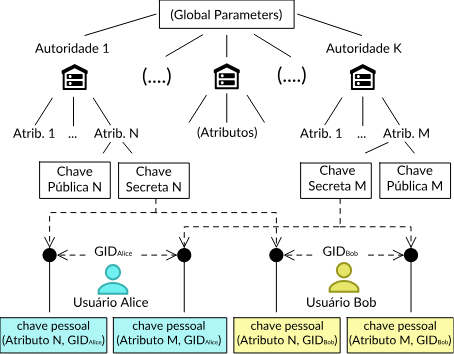
\includegraphics[width=\textwidth]{images/diagrama-DCPABE.png}
  \caption{Um esquema DCPABE com K autoridades e exemplo de geração de chaves pessoais a usuários}
  \label{fig:diagramaDCPABE}
\end{figure}

A figura \ref{fig:diagramaDCPABE} descreve os principais elementos que compõem o esquema DCPABE e a geração de chaves a dois usuários do sistema, Alice e Bob.
Qualquer participante pode se tornar uma autoridade e criar atributos, gerando para cada atributo uma chave pública e uma chave privada, esta última usada para gerar chaves pessoais e intransferíveis aos usuários do sistema.
Esse sistema suporta a escrita de políticas de acesso usando atributos emitidos por diferentes autoridades, tornando-se uma atrativa base fundacional para um sistema de integração criptograficamente seguro.
A fim de impedir ambiguidades, a chave pública de um atributo é considerada a concatenação de seu nome e valor, possibilitando a diferenciação entre dois atributos de mesmo nome gerados por entidades distintas, impedindo também ataques do tipo \emph{spoofing}\footnote{Quando um atacante falsifica informações para se passar por um terceiro com a finalidade de obter acesso ilegítimo no sistema}.
Para impedir ataques de colusão por parte dos usuários, a geração das chaves é feita usando um identificador global \emph{(GID)} de usuário, que é utilizado para "vincular" os atributos de diferentes autoridades a um mesmo usuário. % TODO: (ok) padronizar e diferenciar chave dee identificador no texto todo.
O \emph{GID} é um parâmetro adicional usado durante o processo de verificação da satisfatibilidade da estrutura de acesso no mecanismo de descriptografia e assegura o fracasso do procedimento quando atributos emitidos com \emph{GID} distintos forem utilizados em conjunto para satisfazer uma política de acesso.

A modelagem multi-autoridade da DCPABE é uma solução natural para o problema de compartilhar e integrar dados dispersos entre múltiplas instituições independentes, sem confiança mútua, onde a cooperação possa trazer benefício entre elas.
O comprometimento das instituições participantes consiste somente em fazer a gestão de atributos e utilizar criptografia ABE nos dados passíveis de compartilhamento.
Preserva-se a autonomia dos participantes, uma vez que cabe a eles decidirem as próprias políticas de segurança em termos de ABE e a própria solução para a hospedagem do conteúdo compartilhado. % TODO: (ok) bases de dados de que? explicar melhor
A área da saúde descreve esse tipo cenário, formando uma intrincada rede de serviços ofertados por milhares de instituições no país com as mais variadas características, desde postos públicos de saúde com escopo reduzido a alguns bairros, até hospitais público ou privados, grandes centros de referências de especialidades clínicas, redes de clínicas de exames laboratoriais e centros de pesquisa que colhem dados destas instituições.
A finalidade última é atender ao paciente, e o sucesso do atendimento depende, entre outros fatores, do acesso dos profissionais ao histórico médico deste paciente, entretanto tal histórico está disperso nos diversos prontuários abertos nas instituições pelas quais ele foi atendido no curso de sua vida.
A característica sensível dos dados em prontuários levaram instituições a não correrem o risco de compartilhá-los na internet, não obstante o benefício no atendimento e a obrigação legal de assegurar o acesso do prontuário ao seu dono.

O compartilhamento do histórico de um paciente ocorre normalmente pelo relato oral do paciente quando inquirido pelo médico, sujeito às imprecisões inerentes deste método e, em parte, pela apresentação de alguns documentos aos quais o paciente teve acesso, como por exemplo resultados de exames e laudos.
É comum conseguir o acesso à visualização destes documentos pela internet, mas estes documentos são acessíveis somente ao paciente e somente para visualização, isto é, não é possível que ele exerça controle sobre estes dados para permitir que outros possuam acesso, ou impedir o acesso de alguém a quem a instituição deu a permissão.
Quem atua como a dona dos dados é a instituição, não o paciente, e desta forma é usurpado o direito de propriedade do dono do prontuário aos seus dados.
Um tipo muito mais eficiente de compartilhamento seria obtido se as próprias instituições compartilhassem diretamente os dados dos pacientes, mas isto configuraria um abuso ao direito do paciente enquanto dono das informações contidas no seu prontuário, então seria necessário tornar esse processo sujeito à autorização do dono.
A DCPABE pode devolver o direito de propriedade dos dados ao paciente e possibilitar o compartilhamento seguro de dados entre instituições ao mesmo tempo em que preserva as fronteiras e autonomia das instituições quanto às políticas internas de segurança e de infraestrutura de TI.

{\color{ForestGreen}Explicar um exemplo de uso (1 parágrafo). Pode usar algo assim: https://medium.com/asecuritysite-when-bob-met-alice/towards-true-security-attribute-based-encryption-20d5799aeda6}

Para ilustrar o ponto acima, imagine que é firmado um consórcio entre hospitais e clínicas para disponibilizar consultas a dados de seus pacientes utilizando DCPABE.
Cada hospital participante operaria um esquema ABE, divulgando os atributos que possam ser solicitados e concedendo chaves pessoais aos requerentes, conforme a necessidade.
Neste cenário, suponha que um centro de emergência receba um paciente trazido às pressas resgatado de um acidente, sozinho, inconsciente e que pôde ser identificado a partir dos documentos que portava.
O centro de emergência realiza a consulta em todos os hospitais parceiros do consórcio, e encontram alguns registros referentes ao acidentado.
Cada registro representa um prontuário associado a uma política de acesso definida pela instituição que detém o armazenamento do documento.
As políticas de acesso foram aplicadas pelo próprio usuário pela aplicação disponível a ele, mas poderia também ter sido aplicada pelo hospital com o aval do paciente nos casos em que há dificuldade.
As políticas de acesso acabam todas usando atributos diferentes, emitidos por autoridades diferentes, mas um elemento em comum em todas elas é a presença do atributo ``\emph{emergência}'', conferindo o direito de acesso ao usuário que apresentar uma chave válida deste atributo.
O administrador do centro de emergência tem posse da chave do atributo ``\emph{emergência}'' emitida por cada hospital parceiro e desta maneira tem o acesso aos prontuários que podem auxiliar na tomada de decisão quanto ao caso.
Este cenário privilegia o atendimento de emergência ao considerar a presença prévia do atributo ``\emph{emergência}'' nas políticas de acesso, mas isto não constitui uma obrigatoriedade.
Sem este atributo em um prontuário, este seria aplicado sob demanda, quando por exemplo um hospital recebesse um pedido de acesso ao prontuário junto a uma notificação de internação do paciente, sendo removido das condições de acesso quando tão logo fosse possível delegar a decisão ao paciente ou seu representante legal.

\subsection{Blockchain e Smart Contracts}

{\color{ForestGreen}Explicar quando nasceu, quem a criou e que resolve o problema de não estar atrelada somente a transações financeiras, tendo um uso mais abrangente para qualquer domínio de aplicação. (2 parágrafos).}

Sistemas de pagamentos virtuais surgiram para atender a necessidade do comércio à distância através da internet, e até recentemente esses sistemas estiveram sob custódia exclusivamente de instituições financeiras vistas como entidades confiáveis para a transação de pagamentos eletrônicos.
Neste modelo centralizado, uma autoridade considerada confiável é encarregada da manter a corretude de um sistema, processando as transações dos usuários e rejeitando tanto transações impossíveis (e.g. transações com data passada, saldo negativo ou outros parâmetros incorretos), quanto transações que, embora formalmente válidas, levariam a inconsistências (e.g., transações com gasto duplo).
Sistemas de pagamentos virtuais operam sobre uma ou mais moedas fiduciárias, cada qual sendo emitida pelo sistema bancário de seu país de origem e cuja gestão e controle máximos estão, via de regra, nas mãos de um Banco Central.
Também é atribuído ao sistema bancário a posição de confiança para emissão da moeda, julgando que ele seja imparcial em sua política de expansão ou retração monetária, provendo a liquidez necessária para o mercado
\footnote{Certas escolas de pensamento econômico como a Escola Austríaca \cite{Mises1960, Rothbard2013} criticam a existência de moedas de curso forçado e existência de um Banco central, enquanto defendem a criação e uso de moedas privadas de uso espontâneo. As criptomoedas se tornaram exemplos inesperados desta ideia.}.
Juntamente com corretoras de valores, o sistema bancário e os sistemas de pagamentos eletrônicos são as bases operacionais do mercado financeiro, permitindo o fluxo de capital entre agentes econômicos em escala nacional ou internacional, tornando viável o sistema financeiro mundial como o conhecemos.

Qualquer sistema baseado em confiança tem fragilidades intrínsecas à sua natureza centralizada tais como o abuso hierárquico da autoridade pela imposição de regras arbitrárias, possivelmente invasivas, desnecessárias e ineficientes, a exposição indiscriminada de informações particulares aos membros das autoridades julgadas particulares, a possibilidade de manipulação de transações e taxas do sistema para proveitos particulares e, em um contexto comercial, devido a exigências legais instituídas amplamente que preveem o direito ao estorno de pagamentos, acaba-se introduzindo a possibilidade de perdas permanentes a prestadores de serviços irreversíveis ou produtos perecíveis, abrindo margem para que fraudadores utilizem tais mecanismos para aplicar golpes e obter bens e serviços sem pagar por eles, principalmente em casos onde a mediação de disputas é ineficiente em apurar as reivindicações ou adota um viés que desfavorece o comerciante
\footnote{Veja algumas notícias relacionadas a fraudes \link{https://canaltech.com.br/e-commerce/golpe-pedra-mercado-livre-115288/}{neste}, \link{https://www.techtudo.com.br/noticias/2019/07/golpe-da-compra-falsa-faz-vitimas-no-mercado-livre-veja-como-evitar.ghtml}{neste} e \link{https://www.coindesk.com/how-fraud-sunk-bitcoin-exchange}{neste} link}.
Uma moeda com pagamentos irreversíveis poderia anular o risco de fraude deste tipo, reduzir os custos e estabelecer contratualmente os mecanismos de mediação necessários em caso de disputa.

O \emph{Bitcoin}
\footnote{O termo Bitcoin é utilizado para se referir à unidade de valor utilizada nas transações, à rede de processamento formada pela execução de seu programa e a seus protocolos e tecnologias subjacentes tais como o código e software oficiais.
Desta forma, o sentido do termo pode variar entre moeda, sistema, rede, programa e até plataforma no caso dos sistemas que o utilizem como tal.}
surge como a primeira alternativa viável de uma rede descentralizada ponto-a-ponto de pagamentos que não depende de uma entidade central confiável.
A confiança é depositada aos próprios integrantes da rede de processamento, através de um conjunto de algoritmos e incentivos que, uma vez postos em funcionamento, conseguem produzir o registro válido e imutável das transações, sob a premissa de que a maior parte dos membros da rede não estejam coordenados em um ataque para alterá-lo \cite{nakamoto2008bitcoin}.
Mais importante do que processar pagamentos, o Bitcoin revelou-se um experimento útil para demonstrar a viabilidade de uma ferramenta sem precedentes denominada como \emph{Blockchain}, por meio da qual o consenso distribuído pôde ser obtido.
Já há milhares de soluções
\footnote{Em 03 de outubro de 2020, há mais de mais de 6.200 no site Coinlib e 7.280 projetos registrados no site CoinMarketCap \cite{CoinMarketCap2020, Coinlib2020}, dois dos maiores sites agregadores de informações sobre o mercado de criptomoedas.}
baseadas em Blockchain, que se tornaram conhecidas como \emph{criptomoedas}, embora nem todas elas tenham o objetivo de serem utilizadas primariamente como um sistema de pagamentos, como é o caso da plataforma \emph{Ethereum}, utilizada nesse trabalho.
Entender o conceito de Blockchain é um passo necessário para compreender os fundamentos da mecânica de funcionamento da rede \emph{Ethereum}.

{\color{ForestGreen}Explicar o que é (distributed ledger, cadeia de blocos, transação) e suas características (anonimato, imutabilidade, distribuição). (2 parágrafos).}

Em seu cerne, a Blockchain é uma estrutura de dados com suporte somente à inserção de novos elementos, encadeados por referências ao hash de seu conteúdo, levando portanto a uma quebra da estrutura no ponto em que um elemento seja modificado, impedindo que a modificação passe despercebida e produzindo a propriedade de imutabilidade aos dados, na medida da segurança da função de hashing utilizada. % TODO: (b) redação dá pra ficar melhor
Essa estrutura originalmente foi concebida como uma forma de impor uma ordem cronológica a documentos digitais sem depender da integridade do provedor deste serviço e preservando a privacidade de seus conteúdos \cite{Haber1991}.
A Blockchain é composta por blocos, onde cada um deles referencia o bloco que o antecede, de forma recursiva, até que exista a referência a um bloco especial que inicia essa sequência, denominado como \emph{Bloco Genesis}.
Um bloco é organizado em um cabeçalho e um corpo.
O cabeçalho armazena informações relevantes para a verificação de sua integridade, contendo dados como o hashing do bloco anterior, da árvore Merkle das transações no corpo do bloco, um hashing do próprio cabeçalho, e metadados relevantes como versão do protocolo e parâmetros utilizados para o algoritmo de consenso.
A Figura \ref{fig:blockchain} demonstra essa estrutura.

\begin{figure}[htp]
    \centering
    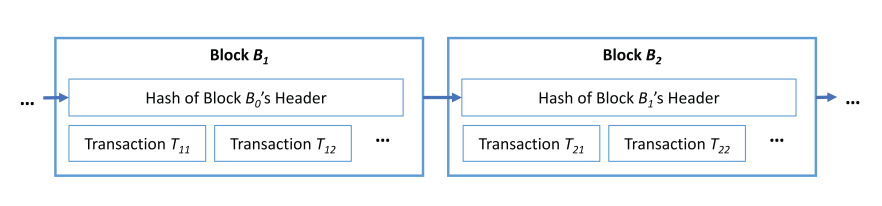
\includegraphics[width=\textwidth]{images/exemplo-de-blockchain.png}
    \caption{Estrutura básica de uma Blockchain}
    \label{fig:blockchain}
\end{figure}

Satoshi Nakamoto projetou a Blockchain do Bitcoin para atender as necessidade de uma moeda, contudo o protocolo extrapola essa finalidade, suportando operações mais complexas, além do simples escopo de um sistema de pagamentos.
Isto porque, ao invés de implementar uma lista preemptiva e exaustiva de todas as transações que pudessem vir a ser necessárias, o protocolo do Bitcoin descreve as transações em termos de comandos de uma linguagem de script baseada em pilha, intencionalmente turing-incompleta, sem loopings ou recursividade, contendo algumas operações aritméticas, lógicas e criptográficas julgadas úteis para oferecer maior liberdade na modelagem de transações que a rede viria a suportar \cite{Narayanan2016a}.

%que impedirá o uso de transações que não o resolvam corretamento e reconhecerá como legítima a transação que a resolver

A transação é a unidade elementar da Blockchain e em sua estrutura possui um cabeçalho contendo metadados e duas listas, denominadas somente como "entradas" e "saídas", que indicam respectivamente de que transação estão vindo os fundos sendo consumidos e qual será a sua destinação.
Uma saída na lista de saídas especifica uma quantidade em bitcoins e usa um script para 'trancar' este valor sob um desafio criptográfico descrito em termos do script do Bitcoin.
Uma entrada na lista de entradas contém uma referência a uma saída específica da lista de saídas de uma transação e um script que "resolve" o desafio relacionado àquela saída.
A checagem de uma transação se dá pela união e execução dos scripts de entrada e saída pelo cliente do Bitcoin, que é considerada válida se, e somente se, para cada elemento da lista de entradas, a execução conjunta dos scripts de entrada e saída resultar em um estado válido, que é definido pelo protocolo como a situação onde, ao fim da execução do script, a pilha de execução do interpretador contar somente com a instrução definida como o valor VERDADEIRO
\footnote{O artigo \cite{Bistarelli2019} ilustra o estado da pilha de um interpretador durante execução de scripts Bitcoin passo a passo.}.
Qualquer outro estado ao final da execução de qualquer um dos elementos de entrada a tornará uma transação inválida e nesta situação será descartada pelos nós da rede Bitcoin que por ventura a receberem.

A linguagem de Script do Bitcoin modela o comportamento das transações e pode ser copiada e reusada em outras transações de mesma natureza.
O script mais utilizado na Blockchain foi chamado de P2PKH \emph{(Pay to Public Key Hash)} e modela uma transação de transferência de moeda Bitcoin entre duas carteiras.
O P2PKH especifica um hash de uma chave pública na saída de uma transação, condicionando a utilização do valor à apresentação da chave pública que corresponda ao hash, juntamente com uma assinatura produzida pela chave privada da respectiva chave pública, permitindo que somente o detentor da chave privada possa utilizar o valor encaminhado a ele por meio da chave pública.
Outros scripts juntamente com este formam um pequeno conjunto de scripts creditados como seguros e alçados ao status de padrão no protocolo do Bitcoin.
Uma transação é considerada padrão quando só utiliza scripts padrões, e mais de 99,9\% das transações na Blockchain são padrões \cite{Bistarelli2019}.
A alta adesão não é coincidência, pois o cliente oficial do Bitcoin não permite a propagação de transações não-padrão pela
rede
\footnote{Não é relevante descrever aqui todas as restrições e validações de transações. É possível ver a lista completa na página da \link{https://en.bitcoin.it/wiki/Protocol_rules\#.22tx.22_messages}{Bitcoin Wiki}},
virtualmente negando o serviço a transações deste tipo, impondo ao seu proponente o ônus de propagar sua transação de forma externa à rede na tentativa de fazê-la alcançar os nós que tenham a eventual chance de incluir um bloco na Blockchain.

Essa linguagem de script demonstra a preocupação desde o projeto do Bitcoin para abarcar, caso fosse necessário, complexidades e regras de transação para além do escopo de uma moeda ou de um sistema de pagamentos, tornando viável projetar por em prática transações de calção, execução de vínculos contratuais, mecanismos de arbitragem privada e transações com multi-assinaturas.
As possibilidades se expandiram no início de 2014 \cite{Greenspan2015} com um \emph{Hard Fork}
\footnote{Hard Fork é uma atualização no protocolo Bitcoin sem compatibilidade com as versões anteriores e que obriga a atualização do software para uma versão compatível com o novo formato dos dados na Blockchain.}
que passou a permitir a adição de até 80 bytes de metadados arbitrários em uma transação, abrindo o caminho, mesmo que limitado, para a utilização da blockchain como um \textbf{livro-razão distribuído} (em inglês, \textbf{\textit{Distributed Ledger}}), isto é, uma fonte de dados capaz de registrar informações de forma imutável e indefinidamente permanente no tempo, com alta disponibilidade, visibilidade pública e acessibilidade.
A \emph{Blockchain 2.0} surge para avançar o suporte a este conceito de livro-razão distribuído, trazendo novas tecnologias baseadas em blockchain, destacando-se as \emph{Smart Properties}, \emph{Smart Contracts} e \emph{DApps (Decentralized Applications)} \cite{Swan2015}.
Essas ferramentas elevam a expressividade e capacidade da Blockchain como uma plataforma para a criação de aplicações financeiras, semi-financeiras, e até mesmo aplicações com ativos que não são financeiros.

%% detalhamento do Bitcoin além do escopo do trabalho removido do texto
% O Bitcoin permite à princípio scripts com tamanho de até 10 mil bytes e com dados de no máximo 520 bytes na pilha de execução\footnote{Informações retiradas do cliente oficial do Bitcoin, versão 0.19, no arquivo de cabeçalho referente a scripts, linhas {\color{RoyalBlue}\href{https://github.com/bitcoin/bitcoin/blob/0.19/src/script/script.h\#L23}{23}} e {\color{RoyalBlue}\href{https://github.com/bitcoin/bitcoin/blob/0.19/src/script/script.h\#L32}{32}}.}.

{\color{ForestGreen}Explicar que para criar o consenso, ou seja, escolher quem irá inserir o último bloco na cadeia, é necessário utilizar o mecanismo de consenso denominado Proof-of-Work (PoW). Explicar em que consiste o PoW. (2 parágrafos).}

%\begin{figure}[!h]
%  \centering
%  \includesvg{images/taxonomia-blockchains.svg}
  %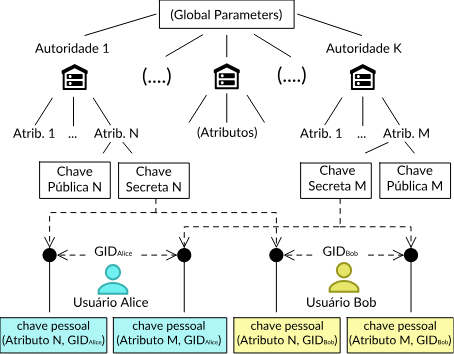
\includegraphics[width=\textwidth]{images/diagrama-DCPABE.png}
%  \caption{Taxonomia de Blockchains quanto ao acesso à rede e diferenciação de usuários}
%  \label{fig:taxonomiaBlockchains}
%\end{figure}

Uma rede Blockchain pode ser configurada como pública ou privada e
pode exigir ou não permissão de entrada.%, formando uma taxonomia ilustrada na figura X.
Uma Blockchain pública disponibiliza seus dados de maneira irrestrita, bastando que o interessado execute o programa para receber os dados difundidos pela rede, sendo o modelo usado em muitas criptomoedas, a exemplo do Bitcoin e Ethereum.
Em decorrência de sua estrutura descentralizada, os projetos de criptomoedas carecem de uma autoridade central para verificar e autenticar usuários e por isso operam em um modelo sem a necessidade de permissão de acesso \emph{(permissionless)}, onde qualquer pessoa pode adicionar nós à rede de processamento.
Redes Blockchain públicas são todas exemplos de de redes sem permissão de acesso e de fato até o momento não há menção de alguma rede do tipo que implemente restrições deste tipo
\footnote{Ruiz\cite{Ruiz2020} propõe uma noção diferente para Blockchains públicas e discute sobre a viabilidade a aplicabilidade deste tipo de rede.}.

Uma Blockchain privada é propriedade de uma instituição ou um consórcio delas com a intenção de incorporar suas vantagens à infraestrutura do setor privado.
Para implantar uma Blockchain privada, pode-se configurar um software da criptomoeda mais apropriada aos requisitos de uso para funcionar em uma rede interna e fechada, ou utilizar arquiteturas desenvolvidas propriamente para este fim, como o Hyperledger Fabric ou Hyperledger Besu \cite{Blummer2019}.
Blockchains privadas são uma opção viável quando instituições sem confiança entre si desejam interagir ou integrar suas bases de dados e ao mesmo tempo não estão dispostas a concordar com uma terceira parte confiável para intermediar a operação deste sistema \cite{OLeary2017, Wust2017}.
O conjunto de participantes é controlado e conhecido, permitindo o uso de identidades para gerenciar o acesso e o direito de escrita na Blockchain.
A leitura de dados pode ser restringida aos participantes ou tornada pública, caso seja vantajoso permitir o acesso a terceiras partes interessadas em realizar a verificação das transações, tais como potenciais clientes, parceiros da cadeia de produção, ou empresas contratadas para realização de auditoria.

A Blockchain do Ethereum e outras criptomoedas operam uma arquitetura p2p e foram projetadas para operar sem a premissa de poder contar com usuários confiáveis para realizar operações sensíveis à rede.
A inexistência de um papel fixo para gerenciar o registro de usuários implica na necessidade de tornar a entrada à rede pública e irrestrita e sem esse controle não é mais possível derivar propriedades de segurança acerca da proporção esperada de usuários que possam ser mal intencionados.
Além do mais, a ausência de diferenciação entre usuários implica em um sistema com homogeneidade de papeis, i.e, um sistema onde todos podem realizar o armazenamento, leitura, escrita e atualização e distribuição dos dados da Blockchain.
A viabilidade da rede depende da correta coordenação entre os usuários em meio a um número desconhecido de usuários desonestos dispostos a subverter a ordem do sistema, formando um cenário equivalente ao descrito na literatura como o Problema dos Generais Bizantinos \cite{Lamport1982}.

É necessário um algoritmo de consenso que coordene as alterações realizadas e estabeleça a frequência em que estas alterações devem ocorrer para que o consenso se propague entre todos os usuários da rede.

O algoritmo de consenso do Ethereum em seu cerne é o mesmo do Bitcoin e resolve esse problema de maneira distinta às soluções presentes na literatura.
O algoritmo de consenso organiza a escrita na blockchain em rodadas, estabelecendo um desafio computacional com uma dificuldade ajustada dinamicamente de acordo com a capacidade de processamento total da rede para que se leve, em média, o mesmo período de tempo para produzir blocos.
A participação desse desafio denomina-se mineração, e os usuários realizando mineração são chamados de \emph{minerador}.
A mineração é uma atividade opcional aos usuários, que podem abrir mão desta tarefa ao configurar seu software para operar no modo \emph{Light node}, somente obtendo dados da rede e realizando a verificação e redistribuição.

O desafio computacional se baseia na ideia do HashCash \cite{Back2002} e foi denominada como \emph{Proof-of-Work} \emph{(PoW)}.
Esse algoritmo estabelece o direito de inserir um bloco na Blockchain para quem apresentar um bloco válido, i.e., um bloco constituído somente por transações válidas e cujo cabeçalho contenha uma solução válida para o PoW.
Uma solução válida para o PoW consiste em um hash cujo valor seja precedido por uma quantidade de zeros de acordo com a dificuldade de mineração estabelecida naquele momento.
A mineração é adversarial uma vez que todos os mineradores estão ao mesmo tempo tentando propor o próximo bloco, e não se sabe quem será o próximo responsável por alterar o estado da Blockchain.

Usuários devem enviar aos outros pares conectados a solução válida de um bloco que serão recebidas, verificadas e redistribuídas até que atinja toda a rede conectada.
A distribuição do novo bloco e sua referência em novas propostas de blocos são o consenso da rede de que ele realmente participa da Blockchain.
Por isso pode-se dizer que o consenso ocorre \textbf{implicitamente}, ou seja, não há coordenação de mensagens para desencadear um processo de decisão formal para que um determinado bloco seja aceito ou rejeitado.
Ao invés disso, o consenso se dá pela inclusão, por meio de sua referência, na cadeia de blocos.

\subsection{Contratos Inteligentes no Ethereum} \label{sec:sub:contratos-ethereum}

{\color{ForestGreen}Explicar para que servem e listar benefícios. (1 parágrafo).}

O conceito de \emph{Smart Contract} antecede o advento da blockchain, vislumbrando a possibilidade de tornar um acordo formal (i.e., um contrato) firmado entre duas ou mais partes em um conjunto de regras computáveis que podem ser, portanto, embutidos no software ou hardware de propriedades com valor e que são controladas por meios digitais, com protocolos estabelecidos para que as partes possam interagir com as regras e desempenhar seus papéis.
Isso possibilita a execução automática do contrato sem a necessidade de intermediários, reduzindo a necessidade de confiança em terceiros e os custos de transação \cite{Bartoletti2019, Szabo1996}.
O Ethereum foi o primeiro e mais bem-sucedido projeto baseado em Blockchain voltado especificamente para a execução de Smart Contracts, fornecendo uma linguagem de programação turing-completa com suporte a funções criptográficas e de consulta de metadados da blockchain, permitindo expressar contratos na forma de programas que podem ser publicados na rede Ethereum e com os quais usuários e outros contratos podem interagir.

Invocações às funções de um contrato se dão por meio de uma transação contendo, entre outros parâmetros, os argumentos para a execução da função e um limite computacional compulsório a esta execução, expresso em termos de um recurso quantitativo denominado \emph{gas}.
O gas é a unidade fundamental do custo computacional na rede Ethereum, é convertido automaticamente a partir do \emph{Ether} --- a moeda base do Ethereum --- e a taxa de conversão é governada por uma equação definida no protocolo da plataforma, levando em conta estatísticas de uso da rede e ajustando o preço da computação de acordo com a demanda registrada na blockchain.
O usuário pode configurar na transação o quanto de gas deseja utilizar, desde que possua o respectivo saldo em Ether, até um limite máximo atribuído pelo próprio protocolo.
Essa mecânica incentiva um uso consciente da capacidade computacional da rede, contorna o problema da indecibilidade quanto ao fim ou não da execução de um programa, impedindo a parada da \emph{Ethereum Virtual Machine (EVM)} diante da execução de funções que, sem tal limitação, ao rodar indefinidamente ou por períodos extensos poderiam perturbar a taxa com que são processadas novas transações, e por fim serve para proteger os recursos do próprio usuário ao interagir com uma função de um Smart Contract cujo custo esteja além da expectativa, quer seja este custo inerente à função (devido à complexidade da operação) ou só produto de um código ineficiente ou mesmo incapaz de terminar.

{\color{ForestGreen}Explicar que a linguagem utilizada é denominada Solidity. Explicar o que é solidity. (1 parágrafo).}

A linguagem na qual Smart Contracts são publicados na rede Ethereum se chama \emph{Ethereum Virtual Machine code (EVM code)} --- uma linguagem de baixo nível baseada em pilhas, similar à linguagem \emph{Forth}.
Visando ampliar o acesso à tecnologia, a Fundação Ethereum desenvolveu também linguagens de programação de alto nível, com sintaxes similares às linguagens mais utilizadas no mercado, com compiladores para produzir EVM code a partir delas. A \emph{Solidity} é uma destas linguagens, com sintaxe similar a Java e C\texttt{++}, dispondo de um compilador com parâmetros configuráveis e um crescente ecossistema composto por padrões de desenvolvimento, bibliotecas e ferramentas de desenvolvimento\footnote{Para se inteirar do ecossistema Solidity, veja \href{https://github.com/bkrem/awesome-solidity}{https://github.com/bkrem/awesome-solidity} ou outras listas publicadas na internet. Entre as bibliotecas, destacam-se a \emph{\href{https://openzeppelin.com/}{OpenZeppelin}}, \emph{\href{https://github.com/dapphub/dappsys}{Dappsys}} e \emph{\href{https://github.com/modular-network/ethereum-libraries}{Modular Libraries}} por atualmente possuírem as maiores bases de usuários, segundo o site \emph{GitHub}.}, destacando-se o ambiente de desenvolvimento e implantação de Smart Contracts \emph{Remix}, utilizada para codificar, depurar e implantar os Smart Contracts do protótipo deste trabalho em redes de teste Ethereum.

{\color{ForestGreen}Explicar o código de um contrato simples que terá o atributo idPaciente, um map de urls de registros médicos e um método addUrl. (1 parágrafo). Explicar que esse contrato é escrito em um arquivo com extensão .sol}

Com Solidity é possível descrever funções e criar variáveis e estruturas de dados, temporárias ou permanentes, que são guardadas na própria blockchain e recuperadas pela EVM conforme a necessidade de uso dos contratos em execução.
A coleção de dados armazenados na Blockchain compõe o que se denomina como estado da EVM.
O código \ref{cod:exemploSmartContract} contém um exemplo de uso de Solidity, implementando um contrato que disponibiliza o acesso de resultado de exames a pacientes.

\lstset{basicstyle=\small, numbers=left, language=bash, keywordstyle=\color{blue}, numbersep=1pt, label={cod:exemploSmartContract}, caption={Exemplo de Contrato Inteligente}}
\begin{lstlisting}
 pragma solidity ^0.5.1;
 pragma experimental ABIEncoderV2;

 contract Hospital {

   enum CodigoResultado {negativo, positivo, inconclusivo, falha}

   struct Registro {
     int version;
     CodigoResultado resultado;
     string data;
     uint MinTime;
     uint MaxTime;
     string extHash;
   }

   mapping (string => Registro) registros;
   mapping (address => string[]) patientURLs;

   function addURL (address patient, string  memory url, Registro memory r) public;
   function getRegistro(string memory url) public view returns (Registro);
  }
\end{lstlisting}

{\color{ForestGreen}Explicar um exemplo passo-a-passo (Só TEXTO, Não Código) de um cliente que obtém o contrato do parágrafo anterior e o executa remotamente em uma máquina. (2 parágrafo).}

As funções implementadas no contrato apontam a existência de dois tipos de papeis relacionados, um que provê informações e outro que as consulta.
O Smart Contract armazena duas tabelas, uma associando endereços a uma lista de URLs e outra associando um URL a um objeto do tipo Registro, que contém as informações de um exame.
Essas tabelas são alimentadas por meio da função \emph{addURL} do contrato, sendo utilizada pelo Hospital que deseja disponibilizar os exames para consulta, e os exames podem ser consultados usando-se a função \emph{getRegistro}.
Ambos os papeis necessitam possuir uma identidade na blockchain Ethereum, ou seja, possuir um endereço válido e ser capaz de publicar transações. Também é necessário possuir um cliente capaz de se conectar a rede para poder publicar novas transações.
Já para a consulta de dados, é possível utilizar serviços Web de terceiros, como sites de visualização de transação, para resgatar uma atualização particular ou obter o estado atual das variáveis do contrato.

Este exemplo, embora introduza a sintaxe da Solidity, também incorre em três situações problemáticas que podem precisar de conserto.
Primeiro, Smart Contracts tem seu código tornado público à rede no momento de sua implantação e suas funções podem ser utilizadas por qualquer usuário com carteira.
Por conta disso, o acesso a funções que alteram o estado do contrato devem impor restrições que verifiquem se o endereço responsável pela interação realmente tem esta prerrogativa.
Geralmente isto se resolve guardando no contrato uma lista de endereços permitidos ou associando-se os dados inseridos no contrato com os endereços de origem e exigir que os dados sejam editados somente por aqueles mesmos endereços.
Segundo, embora a linguagem Solidity disponha de modificadores de acesso para declaração de variáveis, esta modificação só afeta a visibilidade dela por outros contratos, sendo visível e público a quem tiver os da Blockchain Ethereum à disposição.
Isto quer dizer que mesmo com modificadores de acesso privado, os dados não são secretos e podem ser lidos.
No caso do campo \emph{data} no exemplo acima for passível de armazenar informações sensíveis,
No exemplo, caso o campo \emph{data} armazene textos sobre atendimentos, certamente haverão casos em que a informação registrada ali será sensível.
Para resolver este problema, pode-se usar uma função hashing no lugar dos dados, evitando exposição da informação e mantendo disponíveis na Blockchain um verificador para confirmar a integridade deles.
Terceiro e último, mesmo que não configure um problema de privacidade, \emph{data} pode tornar o custo de operação muito alto, uma vez que a escrita de dados permanentes consomem \emph{gas} e as variáveis de tamanho dinâmico são as que mais custam \emph{gas} por cada byte, justamente o caso do campo \emph{data}.
O projeto Ethereum em geral define esta mecânica de custos, junto a outras restrições computacionais, de forma a incentivar o esvaziamento das estruturas de dados nos contratos e a reduzir a quantidade de processamento usado nas funções, tornando vital a divisão de tarefas em módulos distintos, delegando o armazenamento e processamento intensivo de dados a componentes externos, interligados aos contratos.

% -------------------------------------------------------------------- %
\newpage
\section{Sistema Proposto}
\label{sec:sistema-proposto}

\begin{itemize}
    \item {\color{red} Assuma nesta seção que os conceitos de blockchain, Ethereum, contratos inteligentes e criptografia baseada em atributos já foram definidos e explicados.}

    \item {\color{red}Cada parágrafo deve ter em torno de 10 linhas}

    \item {\color{red}Não mostrar código.}

\end{itemize}

\subsection{Visão Geral}
\label{sec:sub:visaogeral}

% {\color{ForestGreen}Explicar que o sistema é composto por X componentes (1 parágrafo).}

A arquitetura do sistema proposto é constituída por 3 módulos: Cliente, Blockchain e Servidor.
Em linhas gerais, o módulo Cliente oferece uma série de funções por linha de comando para a operação do sistema por parte de usuários comuns e certificadores.
O módulo é usado tanto pelos certificadores para criação, publicação e concessão de atributos, quanto pelos usuários para aplicar operações criptográficas utilizando ABE, para publicação dos documentos criptografados na Blockchain e finalmente para realizar o envio e recuperação de dados ao servidor.
O módulo Blockchain é constituído por Smart Contracts que operam de forma autônoma e contínua na Blockchain Ethereum, armazenando diversos dados relacionados a usuários, certificadores, atributos e documentos, processando todas as transações encaminhadas pelo módulo Cliente e realizando verificações adicionais em algumas delas, a fim de garantir a consistência interna dos dados armazenados.
Finalmente, o módulo servidor é responsável por armazenar e distribuir os arquivos criptografados pelo módulo Cliente.

% {\color{ForestGreen}Explicar a função de cada componente (1-2 parágrafos para cada um).}

O módulo cliente é responsável por definir a lógica de funcionamento do sistema, coordenando as atividades dos demais componentes.
Ele acumula funcionalidades que atendem tanto aos usuários do sistema, quanto aos certificadores que outorgam atributos, atributos estes que vão representar basicamente categorias de profissões e instituições as quais os usuários estejam atrelados.
O acúmulo das funções em um único módulo é proposital e objetiva permitir que um usuário possa se tornar um certificador, mas em um escopo reduzido onde não é permitido que os atributos criados por ele possam ser publicados na Blockchain, mas permite-se aplicá-los nos documentos nos quais o usuário for o dono, bem como emitir tais atributos a outros usuários, a fim de possibilitar ao paciente a liberação do acesso de outros usuários não relacionados com o serviço médico (i.e., terceiros de qualquer espécie como conhecidos, familiares, prestadores de serviços como convênios, seguradoras, peritos, etc) ao Prontuário Eletrônico do Paciente (PEP) dele, como será explicado mais adiante na seção \ref{sec:sub:administracao-permissoes}.

O módulo servidor recebe, armazena e envia arquivos criptografados, operando como um serviço Web público na internet.
Este módulo é tratado como um ambiente não-seguro de armazenamento dos dados, sujeito a um possível ataque que leve a acesso não autorizado e roubo de dados, e por esta razão os arquivos enviados a ele estão criptografados.
Para impedir que um atacante ganhe informações por meio de um eventual acesso ilegítimo ao servidor, os arquivos não são vinculados aos dados de identidade do dono, mas a um código gerado de forma aleatória que passa a ser usado como componente de caminho de uma URI para o arquivo.
A comunicação entre cliente e servidor de arquivos segue as seguintes etapas:
\begin{itemize}
  \item solicitar ao servidor, no primeiro envio de um arquivo, a geração de um endereço único para a composição de uma URI;
  \item publicar o endereço da etapa anterior na Blockchain junto aos metadados do arquivo para indicar que o endereço será realmente utilizado pelo usuário para enviar o documento que passa a estar associado a ele pela publicação;
  \item posteriormente, o cliente pode usar o endereço para requisitar o arquivo do servidor e enviar atualizações.
\end{itemize}

O módulo Blockchain consiste em um conjunto de Smart Contracts responsáveis por armazenar diversas estruturas de dados e para impor mecanismos de verificações quanto à validade de transações que levem à inserção ou alteração dos dados lá armazenados.
Existem ao todo oito contratos, descritos na subseção \ref{sec:sub:ImplementacaoSmartContracts}, que conjuntamente tratam da gestão de usuários, certificadores, atributos, requisições para concessão de atributos e documentos.
Os contratos também possuem funções de pesquisa e a recuperação de dados que são utilizados em determinadas operações pelo módulo Cliente para manter a consistência de seu cache local.
Os contratos foram desenvolvidos para operar na rede Ethereum, escolhida principalmente por ser o projeto de criptomoeda pioneiro no suporte nativo à execução de Smart Contracts e por ser o mais bem-sucedido entre as alternativas, considerando como métricas de sucesso o tamanho da comunidade de usuários, de desenvolvedores e a posição relevante ao longo do tempo no mercado de criptomoedas
\footnote{O anexo \ref{app:outrasCriptomoedasSmartContracts} contém uma análise que fundamenta esta afirmação.}.
O ecossistema Ethereum conta com diversas ferramentas, entre elas a biblioteca Web3j, usada nesta trabalho para conectar o código Java com a Blockchain do Ethereum.
A Web3j oferece uma interface Java para o acesso e interação com a Blockchain e permite a geração de classes Java compatíveis com essa interface a partir dos artefatos provenientes da compilação de Smart Contracts.
A Web3j também permite a configuração de diferentes redes compatíveis com o protocolo Ethereum, incluindo a rede principal, as redes públicas de teste ou mesmo uma conexão com uma Blockchain privada local.

% {\color{ForestGreen}Figura dos principais componentes em alto nível: programa cliente (exemplo celular ou notebook), servidor de armazenamento de arquivos; blockchain Ethereum; contratos inteligentes; servidor de chaves de permissões.}

\begin{figure}[H]
  \centering
  \includesvg[width=1.1\linewidth]{images/diagrama-SmartDCPABE.svg}
  \caption{Funcionamento geral e interação entre os módulos cliente, servidor de armazenamento de arquivos e Smart Contracts na Blockchain Ethereum.}
  \label{fig:diagramaSmartDCPABE}
\end{figure}

% {\color{ForestGreen}Explicar um cenário de uso passo-a-passo (exemplo, milestone 1, mas com permissões direcionadas ao contexto de saúde, por exemplo um paciente quer dar permissão de acesso a médicos cardiologistas) (2 parágrafos)}.

A Figura \ref{fig:diagramaSmartDCPABE} apresenta a a relação entre os atores e os módulos em um fluxo de dados partindo da configuração inicial do sistema até o acesso de um arquivo por um usuário.
A linha tracejada entre o Hospital e o Usuário e indica a única transação que ocorre \emph{offline}, isto é, fora do sistema e representa a entrega da chave pessoal de um atributo a um usuário.
As razões para isso são para conservar o escopo deste trabalho e para ater-se ao cenário de uso multi-institucional, cenário que pressupõe uma diversidade de políticas de segurança e privacidade possivelmente incompatíveis entre si, de forma que é sensato deixar esta questão em particular a cargo de cada autoridade certificadora, que então usará os canais que tiver à disposição e que considerar seguro para entrega das chaves.

\begin{enumerate}[label=(\arabic*)]
  \item Um hospital usa o módulo Cliente para atuar como certificadora, gerando uma chave pública de atributo e uma secreta da qual serão derivadas todas as chaves pessoais emitidas aos usuários referente a este atributo.
  \item O certificador utiliza as chaves públicas dos atributos geradas em (1) para aplicar políticas de acesso em um PEP e produz dois arquivos relacionados entre si:
  o primeiro é o próprio PEP, cifrado com AES.
  O segundo arquivo contém a chave utilizada na criptografia AES, que está guardada sob uma cifra ABE definida pela política de acesso associada ao PEP;%, tarefa que pode ser automatizada no caso de uma migração de bases de dados para o sistema proposto;
  \item O certificador envia as chaves públicas dos atributos para o Smart Contract responsável por reunir e disponibilizar as chaves criadas por todas as autoridades em operação;
  \item O arquivo com a cifra do PEP é enviado a um servidor web.
  A confirmação de recebimento gera uma resposta informando um endereço único do arquivo naquele servidor;
  Esta confirmação é registrada, juntamente com a chave AES cifrada com ABE, no Smart Contract responsável pela inclusão, alteração e consulta de documentos disponíveis para os usuários. % TODO: (ok) existe código de acesso, identificador, ficou confuso. Explicar melhor esses conceitos ou padronizar.
  \item O servidor armazena e atualiza os arquivos sem saber seu conteúdo.
  O endereço único do arquivo é um valor aleatório, de forma a anonimizar os dados.
  O servidor opera de maneira RESTful, sem armazenar estados intermediários nas requisições que está processando.
  \item Um usuário pesquisa por arquivos que precise acessar na Blockchain e obtém os metadados deles indicando a política de acesso e o servidor onde está hospedado.
  O documento é recuperado e pode ser descriptografado se o usuário possuir as chaves pessoais dos atributos exigidos.
  Caso o usuário queira salvar alterações no PEP ou a política de acesso, ele deve enviar o novo arquivo ao servidor para a substituição do anterior pelo mais atual e também efetuar a atualização dos metadados que estão registrados no Smart Contract de gestão de arquivos.
\end{enumerate}

A seguir será dado um exemplo de como funciona o sistema.
A paciente Alice recebe um documento digital, correspondendo a seu exame laboratorial de sangue, e deseja adicioná-lo ao sistema.
Para isso, Alice utiliza o módulo cliente para criptografar o documento, usando o esquema ABE, de acordo com uma política de acesso que ela tenha escolhido usar.
Vamos supor que a política escolhida seja a seguinte:

\[paciente \vee (Hospital\textnormal{-}Mario\textnormal{-}Covas \wedge M\acute{e}dico\textnormal{-}Cl\acute{i}nico)\] % (ok) TODO: inserir um nome de um hospital (verificar todas as ocorrências de X)

A política pode ser descrita trocando os símbolos dos operadores lógicos pelo seus nomes em inglês, ou seja, ``paciente OR (Hospital-Mario-Covas AND Médico-Clínico)''.
Ela garante o acesso ao próprio paciente e aos médicos da especialidade Médico Clínico que estejam vinculados ao Hospital Mário Covas
\footnote{O Hospital foi referenciado neste texto somente para fins ilustrativos, e foi escolhido como exemplo pela proximidade geográfica, por ser de gestão pública e pela qualidade dos serviços, conforme certificado pela ONA \cite{ONA2020}.}.
Os atributos possuem múltiplas fontes: o atributo $M\acute{e}dico\textnormal{-}Cl\acute{i}nico$ foi criado pelo CRM do estado de São Paulo, o atributo $Hospital\textnormal{-}Mario\textnormal{-}Covas$ foi criado pelo próprio hospital e o atributo $paciente$ foi criado por Alice.
Alice pôde encontrar os dois primeiros atributos porque eles estão publicados na Blockchain.
O terceiro atributo (paciente) é gerado por todo usuário do sistema e não é publicado como outros atributos criados por certificadores, sendo usado pelo usuário para adicionar à política de acesso uma cláusula que contemple a si mesmo, a fim de permitir o acesso do dono aos próprios documentos.
Embora todo usuário crie e use um atributo de mesmo nome, não existe conflito entre eles porque um atributo é a conjunção de um rótulo e uma chave pública, de forma que a descriptografia só é possível mediante a posse de uma chave pessoal de atributo emitida pelo dono da chave privada usada para a derivação da chave pública gravada no atributo, i.e., somente o emissor do atributo $paciente$ tem as credenciais compatíveis para satisfazer a política de acesso onde o atributo for usado.
% TODO: (ok) a qualquer paciente? Explicar brevemente como o sistema sabe que é ela (Alice) e não qualquer paciente
Repare que a aplicação da política é realizada pelo próprio usuário, efetivamente entregando o controle da segurança da informação ao paciente e respeitando o direito à privacidade da informação.

Após o documento ser criptografado ele está pronto para ser enviado ao servidor.
Para isso, o usuário aciona o módulo cliente, que por sua vez solicita ao servidor de arquivos a geração de um endereço único.
Após a obtenção do endereço, o Cliente envia à Blockchain diversos dados sobre o documento: a identificação do servidor, o endereço único naquele servidor, nome do arquivo, política de acesso, o instante em que a transação está sendo feita e dados produzidos pela criptografia ABE que são necessários no processo de descriptografia do arquivo.
Feita a publicação, o cliente envia o arquivo ao servidor.
Caso não seja o primeiro envio do arquivo\footnote{Um arquivo já existe no servidor se já houver um outro ocupando o endereço informado.}, as etapas de solicitação de endereço e de publicação na Blockchain são puladas, sendo feito somente o envido da nova versão ao servidor, que substitui o arquivo anterior.
Caso a nova versão contenha uma nova política de acesso, o módulo cliente também atualiza a Blockchain para corresponder ao arquivo enviado ao servidor.
Caso o arquivo continue inalterado mas dados a seu respeito na Blockchain precisem de atualização, por exemplo para registrar a migração do arquivo para outro servidor, o módulo cliente também atualizará a Blockchain.

Alice então envia o documento para o servidor de arquivos do Mário Covas e por consequência publica informações sobre o arquivo na Blockchain, entre elas a política de acesso para poder acessar o documento.
Em um segundo momento o Dr. Bob, Médico Clínico do Hospital Mário Covas, ciente de sua agenda com a paciente Alice, está em posse da ficha cadastral dela, onde consta sua carteira Ethereum cadastrada no sistema.
Dr. Bob usa o módulo cliente para consultar por arquivos relacionados ao endereço de carteira Ethereum de Alice e descobre que existe um arquivo compartilhado por ela.
Ele dá o comando para obter o arquivo, levando o módulo cliente a salvar os metadados da Blockchain localmente e realizar uma requisição pelo arquivo em questão ao servidor apontado nos metadados. % TODO: (ok) existe uma relação entre a carteira e o identificador mencionado antes? explicar melhor.
Por último, o Dr. Bob insere o comando para poder acessar o documento e então o módulo cliente usa as chaves pessoais dos atributos possuídos pelo médico para a descriptografia e, uma vez que eles satisfazem a política de acesso, obtém sucesso e o arquivo pode ser visualizado pelo médico.

\subsection{Padronização de Atributos e de Políticas de Acesso}
\label{sec:sub:padronizacao-permissoes}

O sistema proposto oferece aos certificadores a autonomia para a concessão e geração de atributos.
Embora esse modelo descentralizador traga benefícios, também oferece riscos à qualidade da gestão do sistema e da interação entre diferentes instituições.
Sem uma padronização dos atributos, fica a cargo dos usuários compreender a estrutura dos atributos particulares a uma instituição e não há garantia de reaproveitamento deste conhecimento para as outras instituições, porque atributos similares podem ser diferentes entre si no conceito, escopo ou especialização dentro hierarquia definida pelas diferentes profissões exercidas nas instituições e, por outro lado, podem ser similares em tudo isto e diferir apenas no nome.
Por exemplo, enquanto um hospital cria atributos para cada profissão do corpo administrativo do hospital, um outro pode agrupar todos eles em um único atributo ``administrativo''.
Ou, enquanto um emite atributos específicos para cada uma das especialidades médicas existentes, um outro as agrupa em alguns poucos atributos generalizantes.
Em suma, caberiam às instituições decidirem arbitrariamente com quais atributos deveriam trabalhar.
Diferenças quanto às suas competências, especialidades, políticas próprias de acesso à informação e outras normas internas certamente poderiam implicar em arranjos de atributos conflitantes, ao invés de complementares.

Evidencia-se portanto a necessidade de um arcabouço semântico que sirva para coordenar a criação de atributos entre instituições, de forma a assegurar que as políticas de acesso construídas com eles tenham previsibilidade, semântica e funcionalidade preservadas ao longo do tempo.
Para estabelecer este padrão, podemos aproveitar os conteúdos dispostos nas normas que padronizam os Sistemas de Registro Eletrônico de Saúde (S-RES), a forma como são denominados na lei os sistemas de informação na área da saúde.
Esta lista de requisitos é extensa e pode ser encontrada no Manual de Certificação para Sistemas de Registro Eletrônico em Saúde \cite{SBIS2016}.
Em particular, nota-se os requisitos de código \emph{ESTR.09} deste manual preveem que um S-RES deve se submeter aos padrões nacionais e internacionais de representação da informação na área da saúde, definidos como padrão por meio de ato do Ministério da Saúde \cite{MinisteriodaSaude2011}.
Dentre os padrões reconhecidos em lei, o padrão de Troca de Informação em Saúde Suplementar (TISS) \cite{ANS2020} apresenta, entre seus componentes, uma padronização das ocupações na área da saúde, obtidas por sua vez da Classificação Brasileira de Ocupações (CBO) \cite{MTE2010}.

% {\color{ForestGreen}Explicar que foi realizada uma taxonomia das possíveis permissões que seriam utilizadas no sistema para o contexto médico. (3 parágrafos explicando como foi realizado o levantamento, me lembro que tinha um artigo e uma lista gigante que foi filtrada por quantidade de médicos).}

Embora tais normas não tratem diretamente de um cenário onde o controle de acesso à informação seja regido por atributos, pode-se aproveitar a estrutura descrita nelas para desenvolver uma taxonomia das ocupações na área da saúde que se aproxime tanto quanto possível dos padrões em vigor.
Uma taxonomia é uma estrutura classificatória indicando relações lógicas e hierárquicas entre termos de um determinado domínio semântico.
A taxonomia define um vocabulário padrão, o que é útil para a organização da informação, além de permitir que se estabeleçam padrões para alocar, recuperar e comunicar de informações dentro de um sistema de maneira lógica, diminuindo esforços na produção do conhecimento e na sua reutilização \cite{Campos2007}. % TODO: (ok) o texto em vermelho permitirá ao leitor entender o que é taxonomia.
Fez parte deste trabalho propor uma categorização plausível e relevante à área da saúde, que envolveu a análise e agregação de diferentes fontes, tais como o padrão TISS, a CBO e consultas realizadas em sites associados ao Sistema Universal de Saúde (SUS).
A taxonomia fruto deste trabalho consta no Anexo \ref{app:taxonomiaProfissões} e é apresentada de forma resumida na Figura \ref{fig:taxonomiaPermissoes}. % TODO: (ok) no pdf diz Anexo 7 (está errado, deveria dizer Anexo I). Ver como criar anexo (não é como section).
Ela considera mais de 400 profissões distintas, da área da saúde ou fora dela mas relacionadas ao SUS, agrupadas pelo nível de ensino e pelas famílias ocupacionais descritas na CBO.

\begin{figure}[h]
  \centering
  \import{images/}{taxonomia-profissões.tex}
  \caption{Estrutura resumida da taxonomia de profissões da área da Saúde ou relacionadas aos serviços de Saúde}
  \label{fig:taxonomiaPermissoes}
\end{figure}

Pensando em um aspecto ideal de desempenho, deve-se minimizar a quantidade de atributos necessários para representar um papel de um usuário no sistema, ou em outras palavras, deve-se reduzir ao máximo a redundância entre atributos, de forma que haja uma correspondência bijetora entre papéis (profissões) e atributos.
Esta redução de redundância é atingida ao particionar o universo de atributos entre os certificadores, de uma forma tal que não exista superposições entre os papeis representados nestes atributos.
O controle exercido por conselhos profissionais pode servir como base deste particionamento, e assim os atributos descritos na taxonomia que se referem a ocupações regulamentadas por lei seriam administrados pelos conselhos de classe onde tais profissionais precisam ser credenciados ou, na ausência deste tipo de obrigação, pela instituição contratante.
Por exemplo, é obrigatório ao médico possuir credenciamento junto ao CRM da região onde foi formado, portanto o CRM é a indicação natural para se responsabilizar pela emissão de atributos aos médicos formados na região.
Profissionais sem registro em associações de classe (e.g. técnicos administrativos), ou registrados em associações sem cadastro no sistema por não se enquadrarem estritamente na área da saúde (e.g. a CFBio para biólogos ou a CFEP para pedagogos), poderiam ter os atributos referentes às suas ocupações emitidas pelas instituições onde trabalham.

A taxonomia no Anexo \ref{app:taxonomiaProfissões} fornece uma lista exaustiva de todas as ocupações e as agrupa de acordo com as classificações da CBO, onde tanto as ocupações quanto seus agrupamentos podem ser usados como referências para a criação de atributos.
Ainda que isto colabore para a interoperabilidade, não resolve de todo o problema do esquema ABE entre instituições, porque as próprias políticas de acesso carecem de padronização, abrindo margem para a aplicação de condições de acesso arbitrárias, imprevisíveis ou mesmo ilegais.
Além do mais, sem uma normalização das políticas de acesso aos RES, a produtividade dos usuários operando o sistema será prejudicada devido à heterogeneidade das condições de acesso entre instituições, e os custos de automação do sistema serão afetados e aumentarão, porque precisam atuar em muito mais configurações do que quando comparado a um cenário onde existe um conjunto fixo e bem definido de possibilidades.
Por conta disto, além da taxonomia foi desenvolvida um diagrama de condições de acesso ao RES a partir do Código de Ética Médica (CEM) \cite{ConselhoFederaldeMedicina2019}, onde se descreve várias regras e deveres a serem cumpridos por médicos e instituições onde prestam serviço em vários aspectos, entre eles sobre o sigilo do prontuário e das condições de acesso.

% {\color{ForestGreen}Figura da taxonomia}.

\begin{figure}[h]
  \centering
  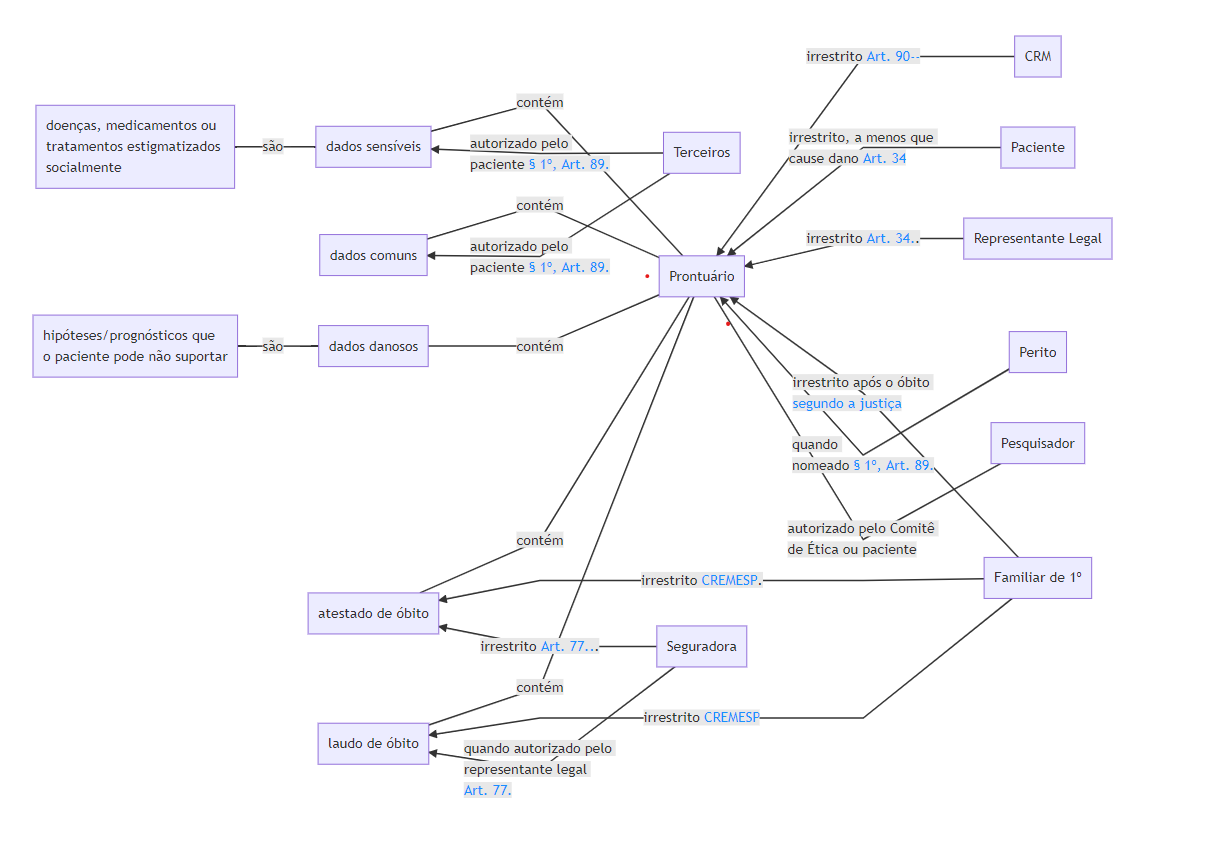
\includegraphics[width=\textwidth]{images/diagrama-de-permissoes.png}
  \caption{Diagrama de permissões de acesso ao Prontuário do Paciente} % TODO: (ok) Essa taxonomia é sua ou do CEM? Se for do CEM, precisa referenciar de onde a obteve
  \label{fig:diagramaPermissoes}
\end{figure}

\begin{table}[h]
  \begin{center}
    \begin{tabular}{ |c|c|c| }
      \hline
      Condição & Escopo & Atores\\
      \hline
      transitória & irrestrito & perito, médico, familiares de 1º grau, pesquisador \\
      \hline
      transitória & restrito & paciente\tablefootnote{Para fins de exemplificação considera-se que o paciente e seu autorizado possuem acesso irrestrito, uma vez que a restrição de acesso para eles provêm de uma exceção à regra, tratada mais adiante no texto}, terceiros, seguradora, pesquisador \\
      \hline
      permanente & irrestrito & CFM, CRM, Representante Legal \\
      \hline
      permanente & restrito & - \\
      \hline
    \end{tabular}
  \caption{Diferentes atores identificados no CEM que podem ter acesso a um prontuário médico.}
  \label{tbl:atores-diagrama-de-permissao}
\end{center}
\end{table}

\begin{table}[h]
  \begin{center}
    \begin{tabular}{ |c|l| }
      \hline
      Natureza da informação & \centerhead{Descrição do conteúdo} \\
      \hline
      comum & dados pessoais e histórico médico em geral. \\
      \hline
      sensível & doenças, medicamentos ou tratamentos estigmatizados socialmente. \\
      \hline
      danosa  & hipóteses ou prognósticos que o paciente pode não suportar saber. \\
      \hline
      legal & atestados e laudo de óbito, podem ser obtidas por terceiros. \\
      \hline
    \end{tabular}
  \caption{Segmentações de um prontuário, derivadas a partir da análise das regras do CEM para acesso ao prontuário médico.}
  \label{tbl:segmentacoes-prontuario}
\end{center}
\end{table}

Foram consideradas nesta análise todas as regras do CEM estipulando condições de acesso a prontuários, resultando no diagrama da Figura \ref{fig:diagramaPermissoes}.
Os atores mencionados no CEM com acesso ao prontuário estão listados na tabela \ref{tbl:atores-diagrama-de-permissao}, agrupados de acordo com a temporalidade e escopo de visualização do prontuário.
O CEM também distingue a naturezas de certas informações dentro do prontuários, aplicando regras diferentes a certos conteúdos, entretanto sem apresentar um modelo formal ou explicitar alguma sistematização quanto a essas partes que compõem o prontuário.
Por isso foi feita a tabela \ref{tbl:segmentacoes-prontuario}, que lista os segmentos observados a partir da diferenciação feita pelos regramentos para o acesso de conteúdos do prontuário, evidenciando naturezas diferenciadas das informações.
Finalmente, o diagrama na figura \ref{fig:diagramaPermissoes} relaciona os agentes da tabela \ref{tbl:atores-diagrama-de-permissao} com o prontuário do um paciente, ou alguma parte dele, representando em suas arestas as condições de acesso às quais os atores estão submetidos.
A partir do diagrama fica claro que as condições de acesso a um prontuário formam um conjunto fixo de regras, a partir do qual pode-se formar, de modo análogo, um conjunto equivalente de políticas de acesso no esquema ABE.
A primeira e mais fundamental política de acesso a ser derivada do diagrama se baseia em todas as regras que instituem acesso irrestrito ao prontuário:

\[ CFM \vee CRM \vee Paciente \vee Terceiro\textnormal{-}Autorizado \]

A justificativa de sua estrutura é simples, afinal usuários como CFM, CRMs, o paciente (dono) e quem for autorizado pelo paciente, por possuírem acesso irrestrito, não devem aguardar a permissão de terceiros ou por acontecimentos que acarretem ao direito de acesso.
A aplicação de uma política de acesso com os atributos ligados de forma disjuntiva garante ao usuário com qualquer dos atributos o acesso imediato aos dados, independente de outras variáveis ou condições, cumprindo efetivamente as condições de acesso irrestrito descritas pelo CEM.
Todas as outras regras definidas pelo CEM são transitórias, como é o caso de um Perito ou Pesquisador, dependentes de algum acontecimento, como é o caso de terceiros que precisam aguardar a autorização do paciente, ou somente se aplicar a uma parte do prontuário, como é o caso de seguradoras e de familiares, que por lei só teriam direito a acessar o atestado e o laudo de óbito
\footnote{Embora a lei não preveja o acesso irrestrito dos familiares ao prontuário do familiar falecido, o diagrama considera esta possibilidade devido a notícias de decisões judiciais em favor disso \cite{G1SE2013}.}.

As regras transitórias de acesso irrestrito diferem do caso anterior somente pela sua restrição temporal, isto é, devem valer somente durante determinado período.
Nesta condição, o usuário buscando autorização de acesso deve comunicar sua necessidade a algum dos atores de acesso irrestrito ao prontuário.
Por exemplo, um perito necessita do acesso ao prontuário para exarar um parecer e pode haver conflitos de interesse do paciente quanto ao resultado da perícia, levando a uma situação onde o paciente ignore a solicitação de acesso feita pelo perito, efetivamente negando o acesso ao prontuário por meio da omissão dele.
Nesta situação, o perito pode solicitar o acesso ao CRM de seu estado, ou ao CFM, que poderão alterar a política de acesso anteriormente descrita para esta:

\[ (Perito \wedge Autorizada\textnormal{-}Per\acute{i}cia\textnormal{-}1) \vee CFM \vee CRM \vee Paciente \vee Terceiro\textnormal{-}Autorizado \]

O perito já possui o atributo $Perito$, emitido a ele pelo certificador representando a Associação onde ele fez credenciamento, por exemplo, a Associação dos Peritos Judiciais do Estado de São Paulo (APEJESP).
Entretanto, se o CRM utilizar somente o atributo $Perito$ na escrita da nova política de acesso, permitirá o acesso não só a ele mas a todos os peritos credenciados na APEJESP.
A solução neste caso consiste em ligar este atributo a um outro específico para esta perícia, neste caso, $Autorizada\textnormal{-}Per\acute{i}cia\textnormal{-}1$.
Desta forma, somente o perito a quem for dada a chave pessoal deste atributo conseguirá ter acesso ao RES.
Cada nova perícia exigiria a publicação de um atributo com numeração específica da perícia, e dependendo da quantidade destas perícias isto pode vir a se tornar a maior parte dos atributos emitidos pelo CRM, que é a instituição responsável por conceder os atributos aos médicos cadastrados no sistema.
Considerando que a quantidade de perícias supera a quantidade de peritos ao longo do tempo, uma alternativa mais eficaz seria criar atributos para identificar os próprios peritos ao invés da perícia, remetendo a ABE a um esquema de uso híbrido, similar à IBE (ver seção \ref{sec:sub:abe}).
Para alcançar uma melhor separação entre conceitos, o CRM deixaria de emitir estes atributos e eles passariam a ser de responsabilidade da Associação de peritos.
Neste cenário onde os atributos identificam os peritos, caberia ao paciente (ou, na omissão deste, ao CRM ou outra autoridade) adicionar o atributo na política de acesso, que ficaria na seguinte forma:

\[ Perito\textnormal{-}1 \vee CFM \vee CRM \vee Paciente \vee Terceiro\textnormal{-}Autorizado \]

Caso $n$ peritos precisem de acesso, podem-se ser acrescentados de forma conjuntiva na fórmula (e.g. $Perito\textnormal{-}1 \vee ... \vee Perito\textnormal{-}n$).
Outro cenário onde há restrição do acesso ao prontuário diz respeito a menores de idade.
A este ponto, é útil salientar que usuários também podem criar e conceder atributos como se fossem certificadores, conforme indicado no exemplo dado ao fim da seção \ref{sec:sub:visaogeral}.
Entretanto, diferentemente dos certificadores, um usuário não publica atributos na Blockchain porque o atributo emitido por ele deve ser usado somente nos próprios documentos, isto é, somente em um escopo de uso local.
É por meio da utilização destes atributos que o usuário garante o acesso ao próprio RES, e também por meio deles que consegue garantir o acesso a terceiros, como está descrito mais a seguir.
Entretanto, para o caso de um menor de idade, não é possível conferir a ele a autonomia sobre a gestão dos próprios dados.
Nesse caso quem fica incumbido da administração do prontuário é o representante legal dele e, para manter a consistência entre nomenclaturas, o atributo criado e usado por ele para esta situação não será $Paciente$, mas sim $Representante\textnormal{-}Legal$. % TODO: (ok) representante legal?
O Representante Legal tem acesso irrestrito ao prontuário do paciente menor de idade, ao menos até a sua emancipação, e a política de acesso nessa situação pode ser escrita na seguinte forma:

\[ CFM \vee CRM \vee Representante\textnormal{-}Legal \vee Terceiro\textnormal{-}Autorizado \]

As políticas de acesso escritas anteriormente consideravam somente o acesso irrestrito ao prontuário, quer seja ele permanente ou temporário.
Um outro tipo de regra prevê acesso parcial ao prontuário, como ocorre com seguradoras, que só podem ver dois documentos específicos, e nada além.
Este tipo de condição de acesso só é possível de ser alcançado se o arquivo do RES possuir uma estrutura modular, onde seja possível percorrer e aplicar diferentes políticas de acesso às suas partes.
Os diversos padrões de sistemas de informação na área da saúde, nacionais e internacionais, exigem que as estruturas de dados de prontuários ou dados clínicos sejam construídas em uma estrutura de árvore \cite{Munoz2011, Dolin2000, SBIS2016, openEHRFoundation2020}, compatível com XML, JSON e outras tecnologias de transmissão e exportação de dados compatíveis com tecnologias Web.
A solução para acessos restritos consiste em aplicar a criptografia não ao arquivo todo, mas às partes que devem conter a permissão específica para o usuário, conforme proposto por \cite{Akinyele2010}.

\begin{figure}[h]
  \centering
  \import{images/}{exemplo-criptografia-modular.tex}
  \caption{Aplicação de políticas de acesso a subelementos de um prontuário}
  \label{fig:exemplo-criptografia-modular}
\end{figure}

O Art. 34 do CEM proíbe que o médico deixe de informar ao paciente sobre o diagnóstico, mas prevê uma única exceção à regra para os casos onde a comunicação direta possa trazer danos ao paciente, como indica o diagrama de condições de acesso na Figura \ref{fig:diagramaPermissoes}.
Suponha por exemplo que um médico evidencia uma piora na saúde mental de um paciente sob seu acompanhamento, a quem deve noticiar sobre um diagnóstico de doença terminal.
O médico julga haver um risco alto e significativo de suicídio frente e decide reter a informação para dá-la a um familiar, ou até que o paciente demonstre condições de suportar toda a verdade.
Para proteger o paciente da informação danosa, o médico precisaria usar o módulo cliente para executar uma transformação nos dados conforme ilustrado na Figura \ref{fig:exemplo-criptografia-modular}.
A seção do arquivo contendo os dados em questão (Fig. \ref{fig:exemplo-criptografia-modular}.a) seria criptografada com uma política de acesso que excluísse o acesso ao paciente, e a cifra resultante do processo seria escrita um nó especial indicando que há conteúdo criptografado (Fig. \ref{fig:exemplo-criptografia-modular}.b).
A descriptografia seria executada de forma recursiva a partir da raíz desta estrutura de dados até suas folhas, e o documento resultante seria o RES composto de nós vazios onde não foi possível o acesso, e de nós com conteúdo, nos elementos onde foi possível realizar a descriptografia por meio dos atributos fornecidos pelo usuário.

Já foi descrito como um usuário pode criar os atributos $Paciente$ e $Representante\textnormal{-}Legal$ para garantir o próprio acesso a um RES dele próprio ou de alguém sob sua tutela. % TODO: esses atributos existem na figura da taxonomia? se não explicar melhor
Para complementar este mecanismo, é possível que um usuário dê acesso a terceiros ao emitir o atributo $Terceiro\textnormal{-}Autorizado$ para eles.
O usuário poderia aplicar este atributo nos mesmos lugares onde aplica o atributo $Paciente$, de forma a garantir o acesso completo ao prontuário, ou aplicar nos mesmos moldes explicados na situação de acesso restrito, onde ele poderia escolher quais partes do prontuário devem ser disponibilizadas aos terceiros.
Estes atributos são geridos pelo usuário porque dizem respeito ao universo pessoal de relações, sendo direito dele exercer seu juízo dos riscos e benefícios do sigilo ou abertura dos próprios dados para outras pessoas ou para conexão com aplicações e serviços de terceiros.

\subsection{Módulo Cliente}

Nesta seção serão apresentadas as diferentes funcionalidades do módulo: geração da taxonomia dos atributos; como são criadas as permissões usando essa taxonomia; como são criptografados os arquivos usando essa taxonomia; como se conectar à Blockchain.

\subsubsection{Administração de Atributos}
\label{sec:sub:administracao-permissoes}
% {\color{ForestGreen}Explicar que o servidor de permissões deverá ser responsabilidade de uma organização apta para entregar as permissões online (ex. Ministério de Saúde ou algúm conselho federal/regional de medicina) (1 parágrafo)}.

A política de acesso a prontuários é aplicada primariamente pelo paciente usando fórmulas lógicas em termos de atributos.
Certificadores são os atores do sistema responsáveis pela criação, publicação e concessão de atributos aos usuários que necessitem deles (e tenham, claro, o direito de solicitá-los).
Os certificadores usam um Smart Contract para disponibilizar os atributos criados por eles aos usuários.
Os usuários consultam por um endereço de carteira Ethereum neste mesmo Smart Contract e obtêm uma lista dos atributos publicados pelo endereço consultado, que pode ser inclusive uma lista vazia, no caso de ainda não existirem atributos publicados por aquele endereço.
Essa estruturação do Smart Contract torna o endereço de carteira Ethereum na identificação primária da instituição certificadora, já que é o meio utilizado para identificar quem é o proprietário de um atributo publicado no sistema.
A fim de permitir a identificação das instituições sem a necessidade de fontes de consulta externas à Blockchain, também há um Smart Contract próprio para a gestão de certificadores e que cataloga estas instituições, associando os endereços de carteira a um nome e contato de e-mail. % (ok) TODO qual operação?
Instituições como o Ministério da Saúde, os Conselhos Federais e Regionais de Medicina, laboratórios, clínicas e hospitais se tornariam certificadores, passando a publicar atributos criados por eles.

Usar endereços de carteira Ethereum como a identidade principal de certificadores evita que um agente mal intencionado forje a identidade de um certificador já cadastrado, uma vez que para se passar por ele o atacante teria que derivar a chave privada a partir do endereço da carteira, o que computacionalmente é muito difícil.
Para publicar atributos, a instituição precisa primeiro ter se registrado junto ao Smart Contract que administra os certificadores.
O sistema proposto trabalha com um cenário sem impedimentos para o registro de novos certificadores.
Entretanto, em um cenário de produção, seria prudente aplicar restrições ao cadastro de novas instituições, adicionando por exemplo uma lista de endereços de administradores para exercer algum tipo de controle nos contratos.
\footnote{Todos os Smart Contracts já contam com funções de uso restrito a um administrador do sistema. Veja a sessão \ref{sec:sub:ImplementacaoSmartContracts:ContratosAuxiliares}, sobre o contrato SmartDCPABERoot}
Em uma solução mais radical, os endereços de administrador seriam os únicos permitidos a usar a função de inclusão de novas instituições.
Uma outra solução, menos restritiva e igualmente viável, é manter a função de cadastro irrestrita, mas exigir a apresentação de uma mensagem assinada por algum dos endereços de administração \cite{Marx2018}, autorizando a entidade a realizar o cadastro.
A mensagem seria pequena, contendo somente o hash de algum dado da instituição, como nome ou endereço de carteira, e o contrato verificaria se a assinatura da mensagem é válida e se o signatário é um dos administradores, efetivando o cadastro da instituição se a entrada estiver correta ou rejeitando, caso contrário.

% {\color{ForestGreen}Explicar que no sistema proposto existe um servidor de atributos ao qual se pedem as chaves públicas/privadas para realizar a encriptação/decriptação (1 parágrafo).}


% {\color{ForestGreen}Explicar como é realizado o passo-a-passo para o pedido/entrega das chaves (note que aqui a descrição é muito mais profunda que o que foi mencionado na visão geral) (1 parágrafo).}

%{\color{ForestGreen}Explicar que a autenticação de uma pessoa para obter a permissão deverá ser realizada de forma externa ao sistema proposto (1 parágrafo).}

Conceder um atributo a um usuário consiste em gerar uma chave única a partir da chave secreta do atributo, em posse do certificador, e do \emph{GID} do usuário.
O módulo cliente permite a geração desta chave somente se for detectada a existência de um pedido registrado na Blockchain por parte do usuário.
O usuário precisa publicar sua requisição de atributos (de um mesmo certificador) em um Smart Contract específico para a gestão de requisições, sendo classificadas como ``pendente'' até que o certificador atualize a situação do pedido.
Só é possível alterar a situação de requisições quando pendentes, efetivamente consumindo a requisição no processo de atualização da situação.
As situações refletem os possíveis resultados de uma requisição e foram padronizadas no mesmo Smart Contract que gerencia as requisições.
Foram definidas as situações ``aprovado'' e ``rejeitado'', de acordo com as possíveis decisões do certificador, e outras poderiam ser criadas para descrever outros cenários a serem implementados como, por exemplo, o caso de uma concessão parcial dos atributos requisitados, ou para detalhar as condições em que uma requisição foi aprovada ou o motivo da rejeição.
A uniformização das situações, o registro público das requisições na Blockchain e a obrigatoriedade da concessão ser feita somente mediante requisição do usuário constituem medidas preventivas visando dificultar a emissão indevida de atributos por parte da instituição certificadora.
Após a geração da chave pessoal de um atributo, cabe ao certificador realizar a entrega de forma \emph{offline} (i.e, fora do sistema), pelas vias que ambos certificador e usuário concordarem ser seguro, como por exemplo e-mail criptografado, serviços web de envio de arquivos ou mesmo pela entrega pessoal da chave em mídia física
\footnote{A implementação de um canal seguro para o envio das chaves pessoais dos atributos foi considerado além do escopo deste trabalho. Isto porque, para o envio dos atributos, as únicas primitivas criptográficas existentes no sistema para formar um canal de comunicação são as chaves geradas pelo Ethereum, pertencentes à curva secp256k1, consideradas inseguras para o uso em criptografia assimétrica \cite{Bernstein2017}. Seria necessário, portanto, o uso de outro protocolo, não relacionado ao tema principal deste trabalho.}.

% Após a autoridade gerar uma chave pessoal do atributo, esta é encaminhada ao usuário de forma externa ao sistema (e.g., via correio eletrônico, que terá no conteúdo um link seguro para baixá-la)., eliminando desta forma a existência de outros algoritmos e chaves que não fossem relacionados ao trabalho.
%Teoricamente seria possível criar um canal seguro entre usuários sem a adição de outros algoritmos e chaves distintas das já utilizadas uma vez que o Ethereum cria um par de chaves que poderiam ser usadas como chaves assimétricas em um sistema de criptografia de curva-elíptica \emph{(Elliptic-Curve Cryptography - ECC)}, porém tal investigação está além do escopo deste trabalho\footnote{O par de chaves pública e privada geradas pelo Ethereum pertence à curva secp256k1, que não é considerada segura.
%Estudar um sistema com essa capacidade envolveria em primeiro lugar a escolha de uma blockchain alternativa compatível com as curvas consideradas seguradas para realizar a ECC \cite{Bernstein2017}.}. % TODO: (ok) por enquanto vamos deixar de lado essa parte da segurança, pois está fora do contexto da seção que fala de taxonomia.

%O sistema proposto integra bases de dados de diferentes órgãos que, quando tornados  certificadores, serão providos com a capacidade de publicar tantos atributos quanto considerarem necessários.

Em resumo, o fluxo da requisição por um atributo, isto é, da requisição das chaves pessoais daquele atributo para um usuário funciona da seguinte maneira.
Primeiro, o módulo cliente realiza uma requisição de um atributo, publicando-a na Blockchain.
Esta requisição contém uma situação, uma lista de atributos (neste exemplo, um só) e o endereço do certificador responsável por elas.
Em um segundo momento, o certificador desse atributo consulta a Blockchain para obter as requisições e decide se irá processá-las ou não.
A seguir, ele atualiza a situação da requisição na Blockchain de acordo com uma lista possível de situações, informando se aceitou ou rejeitou por meio dos códigos disponíveis na Blockchain.
Finalmente, o usuário usa o módulo client para checar a Blockchain, a resposta é recebida e se ela for positiva, caberá ao usuário e certificador acordarem a forma de envio da chave pessoal do atributo.
Cabe destacar que quaisquer operações criptográficas envolvendo chaves sempre ocorrem localmente e que chaves nunca são transmitidas pela rede para evitar a exposição de informação sensível.

\subsubsection{Criptografia com ABE}
\label{sec:sub:criptografia-abe}

% {\color{Magenta} 1 parágrafo para explicar que para encriptar um documento utilizando atributos usou a dcpabe.}

A biblioteca DCPABE desenvolvida em Java possui suporte à operações criptográficas do protocolo ABE em um ambiente com múltiplas autoridades, conforme descrito em \cite{Lewko2011}.
Por sua vez, ela depende da biblioteca \emph{jPBC} (Java Pairing Based Cryptography) \cite{DeCaro2011} para realizar a criptografia baseada em emparelhamento
\footnote{mais informações em \href{https://crypto.stanford.edu/pbc/}{https://crypto.stanford.edu/pbc/}}.
A DCPABE fornece todas as ferramentas necessárias para o uso do esquema ABE, incluindo a geração de parâmetros globais, geração de chaves privadas, públicas e pessoais dos atributos e operações criptográficas. % TODO: (ok) manter (padronizar) a mesma palavra (decifrar, decriptar, descriptografar) no texto todo.
Ao criptografar um documento, um objeto do tipo \emph{Ciphertext}, contendo os parâmetros necessários para a descriptografia, é serializado e escrito no início de um arquivo que conterá os bytes criptografados.
Esse comportamento da biblioteca foi modificado no protótipo deste trabalho para que a criptografia serializasse o objeto \emph{Ciphertext} em um arquivo JSON, para ser publicado na Blockchain.

% {\color{Magenta} 1 parágrafo para explicar as 3 linhas mais importantes do código fonte de como realizar a encriptação. Explicar cada linha do código.}

\lstset{basicstyle=\small, numbers=left, language=java, keywordstyle=\color{blue}, numbersep=1pt, label={cod:metodoCriptografia}, caption={Criptografando um arquivo usando a biblioteca DCPABE}}

\begin{lstlisting}
 public void encrypt(String file, String policy, String[] authorities) {
   // codigo omitido por brevidade
   AccessStructure as = AccessStructure.buildFromPolicy(policy);
   Message m = DCPABE.generateRandomMessage(gp);
   CiphertextJSON ct = new CiphertextJSON(DCPABE.encrypt(m, as, gp, pks));
   r = new Recording(path, file, ct);
   r.encryptFile(m);
 }
\end{lstlisting}

No sistema, a classe \emph{Client} implementa a função que realiza a criptografia de um arquivo (função \emph{encrypt}), em parte exposto seção de código \ref{cod:metodoCriptografia}.
A função encrypt exige os parâmetros \emph{file}, que corresponde ao nome do arquivo a ser criptografado; \emph{policy}, que corresponde à política de acesso; e o vetor \emph{authorities}, que corresponde aos IDs das autoridades dos atributos definidos em \emph{policy}.
Na linha 3, o objeto \emph{as}, instância da classe \emph{AccessStructure}, armazena uma representação matricial da fórmula booleana descrita em \emph{policy}, usada pela DCPABE para a criptografia.
Na linha 4 a mensagem \emph{m} é definida como um elemento aleatório pertencente ao grupo do aparelhamento definido pelos parâmetros globais \emph{gp} -- o mesmo utilizado para a geração de chaves privadas dos atributos.
A mensagem \emph{m} é a informação que de fato é criptografada com ABE, enquanto que no arquivo  a criptografia ocorre usando \emph{m} como uma semente para um algoritmo de cifra AES\footnote{Especificamente, é usada a classe AESEngine da biblioteca Bouncy Castle com configuração padrão. Ver \href{https://people.eecs.berkeley.edu/~jonah/bc/org/bouncycastle/crypto/engines/AESEngine.html}{https://people.eecs.berkeley.edu/~jonah/bc/org/bouncycastle/crypto/engines/AESEngine.html}}, conforme pode ser visto na linha 7.
Na linha 5 a mensagem m é ocultada sob a criptografia ABE utilizando a matriz \emph{as}, a mensagem \emph{m}, os parâmetros globais \emph{gp} e um vetor \emph{pks} com as chaves públicas de todos os atributos mencionados em \emph{policy}, retornando uma instância serializável da classe \emph{Ciphertext}.

A ABE não permite a criptografia de tamanho indiscriminado, e uma forma de resolver isso é usando um algoritmo sem esse tipo de limitação para criptografar o arquivo e criptografar a chave usada (neste caso, \emph{m}) pela aplicação da ABE.
Por outro lado, a descriptografia consiste em fornecer as chaves pessoais dos mesmos atributos usados na criptografia, aplicando o esquema ABE para obter a mensagem \emph{m} e usando-a como chave do algoritmo AES para descriptografar o conteúdo desejado.

% {\color{Magenta} 1 parágrafo para explicar as 3 linhas mais importantes do código fonte de como decriptar um arquivo. Explicar cada linha do código.}

\subsubsection{Conexão com a Blockchain e acesso aos \textit{Smart Contracts}}

% Como mencionado na Seção \ref{sec:sub:visaogeral}, o sistema é composto por 3 componentes: cliente, servidor, e a Blockchain. %A Figura X mostra o relacionamento entre esses componentes.

%{\color{ForestGreen} Fazer uma figura simples que mostre os 3 componentes interligados. }


%{\color{ForestGreen} Explicar implementação do cliente (5 parágrafos). Ver abaixo os 5 parágrafos destrinchados. }

%{\color{Magenta} 1 parágrafo para explicar que para realizar a conexão com a Blockchain usou o web3j (explique em 2-3 linhas o web3j).}

Como mencionado, o Cliente precisa conectar-se à Blockchain para realizar suas atividades.
Em se tratando da conexão, a biblioteca Web3j fornece conectividade com diferentes fontes de dados para consulta (do estado das transações e envio de novas transações) em Blockchains compatíveis com o protocolo JSON-RPC Ethereum
\footnote{ver \href{https://github.com/ethereum/wiki/wiki/JSON-RPC}{https://github.com/ethereum/wiki/wiki/JSON-RPC}.}.
Entre essas fontes, podem-se citar a rede principal (denominada \emph{MainNet}), as redes de teste oficiais (Ropsten, Rinkeby e Kovan) ou simulações da rede Ethereum para teste por meio de programas como o Ganache~\cite{Ganache2020}.
% A Web3j se conecta ao provedor de dados por meio de Protocolos HTTP/HTTPS e IPC.

\lstset{basicstyle=\small, numbers=left, language=java, keywordstyle=\color{blue}, numbersep=1pt, label={cod:conexaoBlockchain}, caption={Código para conexão com a Blockchain usando o web3j}}

\begin{lstlisting}
 private final Web3j web3j;

 public BlockchainConnection(String networkURL, ...) {
   // codigo omitido por brevidade
   web3j = Web3j.build(new HttpService(networkURL));
 }
\end{lstlisting}

% {\color{Magenta} 1 parágrafo para explicar as 3 linhas mais importantes do código fonte de como realizar a conexão. Explicar cada linha do código. }

No sistema proposto, a conectividade é realizada no módulo Cliente.
Dentro desse módulo, a classe \emph{BlockchainConnection} é a responsável por lidar com a Blockchain (por meio do Web3j) e com as classes em Java que representam os Smart Contracts. Como mostra o código \ref{cod:conexaoBlockchain}, para realizar o acesso  somente é exigido um endereço IP/porta válido (atributo networkURL) no computador ou rede local onde exista comunicação com a API JSON-RPC do Ethereum, ou com um serviço Web que ofereça essa API, tais como os sites da Infura e do Ethercluster.
%O endereço informado é armazenado no cache do programa para uso em execuções futuras.

% {\color{Magenta} 1 parágrafo para explicar as 3 linhas mais importantes do código fonte de como acessar um contrato inteligente. Explicar cada linha do código.}

\lstset{basicstyle=\small, numbers=left, language=java, keywordstyle=\color{blue}, numbersep=1pt, label={cod:acessoSmartContract}, caption={Acessando um Smart Contract na Blockchain}}

\begin{lstlisting}
 private CiphertextJSON getCiphertext(String user, String fileName) {
   Tuple5<String, byte[], byte[], byte[], byte[]> ciphertextData;
   try {
     ciphertextData = contractFiles.getCiphertext(user, fileName).send();
     if (!ciphertextData.getValue1().equals("")) {
       // codigo usando os dados retornados pelo contrato
     }
   } catch (Exception e) { ... }
 }
\end{lstlisting}

O acesso aos Smart Contracts em Java é intermediado por classes "wrappers", isto é, classes geradas automaticamente a partir do EVM Code e da ABI \emph{(Application Binary Interface)} de Smart Contracts para interação com o contrato.
Estas classes contém métodos que correspondem às funções nos Smart Contract, possuindo dois métodos a mais, um para implantar o contrato na EVM e outro para carregar o contrato, caso já tenha sido implantado.
Uma vez inicializado, a interação ocorre como exemplifica a sessão de código \ref{cod:acessoSmartContract}.
Na linha 4 o método \emph{getCiphertext} do objeto \emph{contractFiles} (wrapper do contrato \emph{SmartDCPABEFiles}) recebe os argumentos necessários, prepara um objeto que representa uma chamada remota ao contrato, e o envia à rede Ethereum por meio da invocação do método \emph{send()} ao fim da linha.

As funções executadas nos Smart Contracts podem retornar dados, sendo inseridos em um objeto do tipo \emph{TupleN}, onde N o número de parâmetros retornados. Este objeto possui métodos na forma \emph{getValueN()} para acessar o n-ésimo valor de retorno do Smart Contract.
A checagem feita na linha 5 é necessária para identificar se o objeto retornado pelo Smart Contract é vazio.
Isto é necessário porque a implementação da EVM não possui um elemento nulo como na maioria das linguagens, e também não levanta um erro quando tenta-se acessar um valor inexistente.
Quando a EVM acessa uma variável indefinida ou inexistente, seu comportamento padrão é retornar um valor do mesmo tipo da variável que corresponda ao valor FALSO de uma variável booleana.
Assim, sem um mecanismo de erro ou identificação de valores nulos, torna-se necessário checar o valor de alguma das variáveis recebidas cujo valor não possa ser equivalente ao FALSO booleano.
No código \ref{cod:acessoSmartContract}, a variável escolhida é \emph{policy}, que ocupa a posição 1 da tupla e que nunca pode ser igual a uma string vazia, visto que isto significaria que o conteúdo não está criptografado, necessariamente significando que o valor de retorno se refere a valores nulos ou inexistentes.
Confirmado que os dados recebidos realmente existem, estes são processados no escopo aninhado à verificação, na linha 6.

\subsection{Módulo Blockchain}

Nesta seção serão apresentados detalhes sobre as estruturas de dados e algumas funções principais nos Smart Contracts ligados à lógica principal do protótipo.
A seguir há uma documentação sobre os elementos do ecossistema Ethereum utilizados neste trabalho e por fim a seção encerra com detalhes de implantação dos Smart Contracts na testnet Rinkeby.

\subsubsection{Contratos Inteligentes}
\label{sec:sub:ImplementacaoSmartContracts}

Foram desenvolvidos cinco contratos inteligentes que que permitem realizar a autenticação, entrega de permissões e armazenamento de metadados dos prontuários eletrônicos dos pacientes.
A seguir serão explicados cada um deles.

\textbf{Contrato SmartDCPABEAuthority}

%{\color{ForestGreen} Explicação do  SmartDCPABEAuthority (3 parágrafos). Ver abaixo os 3 parágrafos destrinchados.}

% {\color{Magenta} 1 parágrafo para explicar o que faz o contrato (em linhas gerais).}

O contrato \emph{SmartDCPABEAuthority} registra na Blockchain as entidades certificadoras disponíveis no sistema, associando dados de identificação e a quantidade de atributos que a entidade já publicou a um endereço de carteira que será creditado como dela no ato do cadastro.
A publicação na Blockchain garante um mecanismo descentralizado de cadastro, com disponibilidade contínua.
A chave privada associada ao endereço de carteira Ethereum é utilizada como valor do \emph{GID} na geração das chaves públicas e privadas dos atributos no esquema ABE.
Essa escolha é feita para assegurar que todo certificador possua um endereço Ethereum e para provocar um vínculo entre sua identidade na Blockchain e sua atuação como certificador, de forma que não seja possível a um atacante forjar a identidade de um certificador pela cópia de dados públicos de identificação, sendo necessário que descubra a chave privada associada à carteira, ou que a derive a partir do endereço de carteira, tarefa que até o momento se demonstra computacional inviável
\footnote{Essa inviabilidade computacional presume que a chave foi gerada usando um processo aleatório seguro. Caso não use, a chave estará suscetível a ataques, veja por exemplo \cite{Bednarek2019}.}.
% TODO: (ok) unidades? que unidades? se for instituição ou entidade padronizar no texto todo

%{\color{Magenta} Inserir o código da linha 7 até 20.}

\lstset{basicstyle=\small, numbers=left, language=bash, keywordstyle=\color{blue}, numbersep=1pt, label={cod:SmartDCPABEAuthority}, caption={Dados em SmartDCPABEAuthority}}
\begin{lstlisting}
 contract SmartDCPABEAuthority is Collection {

 struct Certifier {
   address addr;
   bytes32 name;
   bytes32 email;
   uint64 numPublicKeys;
 }

 address[] public certifierAddresses;
 mapping (address => Certifier) certifiers;
\end{lstlisting} % TODO: (meio-ok) parágrafo explicando cada um dos atributos. Exemplo: o atributo addr permite identificar unicamente o certificador que cria os atributos. O atributo name corresponde ao nome dele (e.g., ...)

% {\color{Magenta} 1 parágrafo para explicar para que serve CADA UM dos structs, events e atributos. Exemplo. O struct X permite armazenar dados que servirão para Y. O atributo V armazena informações de W que servirão para Z.}

A sessão de código \ref{cod:SmartDCPABEAuthority} exibe os pontos mais relevantes do contrato.
A estrutura (\textit{struct}) Certifier armazena dados informações da autoridade responsável por publicar atributos e concedê-los a usuários.
Além do endereço Ethereum, também é armazenado seu nome, e-mail e a quantidade de chaves que ele já publicou.
Tal unidade de controle é necessária porque as chaves são armazenadas em \emph{mappings}, conforme explicitado na Sessão \ref{sec:sub:contratos-ethereum}.

\textbf{Contrato SmartDCPABEKeys}

%{\color{ForestGreen} Explicação do  SmartDCPABEKeys (3 parágrafos). Ver abaixo os 3 parágrafos destrinchados.}

% {\color{Magenta} 1 parágrafo para explicar o que faz o contrato (em linhas gerais).}

O contrato \emph{SmartDCPABEKeys} disponibiliza a chave pública de atributos criados por autoridades.
No sistema, foram implementadas somente as operação de inclusão e consulta de chaves, mas não de edição ou remoção.
Cabe destacar que não seria complicado implementar isto no Smart Contract.
Por outro lado, não seria fácil implementar os protocolos de revogação e substituição de atributos no módulo Cliente.%, responsável pelas operações criptográficas e pela coordenação das informações entre a Blockchain e o Servidor.

% {\color{Magenta} Inserir o código da linha 6 até 24.}

\lstset{basicstyle=\small, numbers=left, language=bash, keywordstyle=\color{blue}, numbersep=1pt, label={cod:SmartDCPABEKeys}, caption={Dados em SmartDCPABEKeys}}
\begin{lstlisting}
 contract SmartDCPABEKeys is Collection {

 struct PublicKey {
  Bytes127 eg1g1ai;
  Bytes127 g1yi;
 }

 struct Bytes127 {
  bytes32 chunk1;
  bytes32 chunk2;
  bytes32 chunk3;
  bytes31 chunk4;
  uint8 lastChunkSize;
 }

 mapping (address => bytes32[]) publicKeyNames;
 mapping (address => mapping (bytes32 => PublicKey)) ABEKeys;
\end{lstlisting}

% {\color{Magenta} 1 parágrafo para explicar para que serve CADA UM dos structs, events e atributos.}

A sessão do código \ref{cod:SmartDCPABEKeys} exibe os pontos mais relevantes do contrato.
A estrutura \emph{Bytes127} foi criada como um contêiner que armazena os elementos gerados pela biblioteca jPBC \emph{(Java Pairing-Based Cryptography)} \cite{DeCaro2011}. % TODO: (meio-ok) que elementos? (explicar antes ou no capítulo correspondente)
O tamanho dos elementos varia entre 120 a 124 bytes de informação e, embora o Solidity disponha da estrutura de dados \emph{bytes} para armazenar bytes em tamanho arbitrário, seu custo é maior.
Dados consomem gas, e quando são utilizadas estruturas de dados de tamanho dinâmico, o valor é maior do que suas contrapartes estáticas, justificando a criação de uma estrutura que divida os dados em um conjunto de elementos de tamanho fixo.
A estrutura \emph{PublicKey} armazena a chave pública gerada pela biblioteca \emph{DCPABE}\footnote{código fonte: \href{https://github.com/stefano81/dcpabe}{\texttt{https://github.com/stefano81/dcpabe}}. Para uma análise teórica, ver \cite{Lewko2011}}, que são representadas por duas sequências de bytes como mostra o código.
O mapa \emph{publicKeyNames} mapeia um endereço de uma autoridade a uma lista de nomes de atributos, representados como bytes.
O mapa \emph{ABEKeys} contém, para cada endereço cadastrado, um submapa relacionando o nome do atributo, representado em bytes, com uma chave pública.

\textbf{Contrato SmartDCPABEFiles}

%{\color{ForestGreen} Explicação do  SmartDCPABEFiles  (3 parágrafos). Ver abaixo os 3 parágrafos destrinchados.}

% {\color{Magenta} 1 parágrafo para explicar o que faz o contrato (em linhas gerais).}

O contrato \emph{SmartDCPABEFiles} mantém disponível na Blockchain informações sobre a hospedagem (localização) do arquivo e também os dados do objeto \emph{Ciphertext} produzido pela Biblioteca DCPABE, necessário para realizar a descriptografia.
O contrato também gerencia informações sobre as bases de dados onde os arquivos estão hospedados.

% {\color{Magenta} Inserir o código da linha 6 até 39.}

\lstset{basicstyle=\small, numbers=left, language=bash, keywordstyle=\color{blue}, numbersep=1pt, label={cod:SmartDCPABEFiles}, caption={Dados em SmartDCPABEFiles}}
\begin{lstlisting}
 contract SmartDCPABEFiles is Collection {

 struct Recording {
  uint64 serverID;
  bytes32 key;
  bytes32 hashing;
  uint64 timestamp;
 }

 struct Ciphertext {
  string policy;
  bytes c0;
  bytes c1;
  bytes c2;
  bytes c3;
 }

 struct FileServer {
  bytes32 domain;
  bytes32 path;
  uint16 port;
 }

 uint64 public numServers;
 mapping (address => string[]) fileNames;
 mapping (address => mapping(string => Recording)) files;
 mapping (address => mapping(string => Ciphertext)) ciphertexts;

 FileServer[] servers;
\end{lstlisting}

% {\color{Magenta} 1 parágrafo para explicar para que serve CADA UM dos structs, events e atributos.}

A sessão do código \ref{cod:SmartDCPABEFiles} exibe os pontos mais relevantes do contrato.
A estrutura \emph{Recording} informa a base de dados na qual o arquivo está hospedado e, no campo serverID, qual é a sua identificação no servidor.
O campo hashing permite a verificação de integridade.
O campo timestamp é uma marca temporal que mantém o momento de sua publicação na Blockchain. %Seria possível remover o campo timestamp e trabalhar somente com altura ou timestamp do bloco em que a transação foi validada, economizando o uso de gas, porém deixando de possuir uma data exata de publicação de um documento.

A estrutura \emph{Ciphertext} contém a política de acesso utilizada para criptografar o arquivo e um conjunto de parâmetros (c0 a c3) que resultam do processo de criptografia e que são necessários para descriptografar o documento.
A estrutura \emph{FileServer} contém informações para conexão com uma base de dados na Internet.

Além das estruturas, o contrato mantém uma lista de servidores \emph{servers} e um par de mapas \emph{files} e \emph{ciphertexts} com estrutura similar, mapeando endereços de usuários a submapas que associam, por sua vez, um nome de arquivo às estruturas de dados \emph{Recording} e \emph{Ciphertext} relacionadas àquele arquivo. %Disso segue-se que uma edição no conteúdo é mais barato que a alteração no nome do documento, uma vez que no caso do conteúdo somente o hashing e o timestamp são atualizados, enquanto que na renomeação o mapa armazena o arquivo como se fosse um novo, sendo necessário publicar os dados do arquivo e deletar aqueles que estavam disponibilizados.

\textbf{Contrato SmartDCPABERequests}

%{\color{ForestGreen} Explicação do  SmartDCPABERequests  (3 parágrafos). Ver abaixo os 3 parágrafos destrinchados.}

% {\color{Magenta} 1 parágrafo para explicar o que faz o contrato (em linhas gerais).}

O contrato \emph{SmartDCPABERequests}  é responsável por lidar com requisições de concessão de atributos.
Usuários do sistema publicam suas requisições e as autoridades certificadoras podem checar por requisições pendentes e atendê-las ou rejeitá-las.
Uma requisição pode solicitar a concessão de um ou mais atributos a um mesmo certificador e é consumida quando processada, não sendo possível alterar novamente seu status.
A transmissão dos atributos ocorre fora da Blockchain e pode usar qualquer meio de comunicação considerado seguro entre as partes.

% {\color{Magenta} Inserir o código da linha 6 até 35.}

\lstset{basicstyle=\small, numbers=left, language=bash, keywordstyle=\color{blue}, numbersep=1pt, label={cod:SmartDCPABERequests}, caption={Dados em SmartDCPABERequests}}
\begin{lstlisting}
 contract SmartDCPABERequests is Collection {

 enum KeyRequestStatus {
  PENDING,
  OK,
  REJECTED
 }

 struct KeyRequest {
  KeyRequestStatus status;
  uint64 timestamp;
  uint64 responseTimestamp;
  bytes32[] attrNames;
 }

 event pendingRequestIndexChanged(uint64 oldIndex, uint64 newIndex);
 event pendingRequesterIndexChanged(uint64 oldIndex, uint64 newIndex);

 mapping (address => address[]) pendingRequesters;
 mapping (address => mapping (address => uint64[]))  pendingRequests;
 mapping (address => mapping (address => KeyRequest[]))  requests;
\end{lstlisting}

% {\color{Magenta} 1 parágrafo para explicar para que serve CADA UM dos structs, events e atributos.}

A sessão do código \ref{cod:SmartDCPABERequests} exibe os pontos mais relevantes do contrato.
A estrutura \emph{KeyRequest} representa uma requisição de atributos, contendo um campo para indicar a situação (enum das linhas 3-7), marcas temporais da criação e processamento da requisição e uma lista de nomes de atributos representados como sequências de 32 bytes (Bytes32).
As situações estão listadas no enum \emph{KeyRequestStatus}, e podem ser expandidas para um conjunto maior de situações, conforme a necessidade das entidades que utilizem o sistema.
Dois eventos notificam sobre o processamento de requisições, para que os interessados possam obter  o estado mais atualizado das requisições.
O mapa \emph{requests} usa endereços de certificadores como chave primária para submapas cujas chaves são os endereços de usuários e que mapeiam às listas de requisições feitas por eles.
O mapa \emph{pendingRequests} segue esta mesma estrutura, com a diferença de apenas armazenar os índices das listas de requisições em \emph{requests} que estão pendentes de processamento.
O mapa \emph{pendingRequesters} mantém os endereços de usuários com requisições pendentes em listas agregadas por certificador, possibilitando que estes possam iterar pelo mapa \emph{pendingRequests}, obtendo os índices de acesso das requisições de interesse gravadas em \emph{requests}.

\textbf{Contrato SmartDCPABEUsers}

%{\color{ForestGreen} Explicação do  SmartDCPABEUsers  (3 parágrafos). Ver abaixo os 3 parágrafos destrinchados.}

% {\color{Magenta} 1 parágrafo para explicar o que faz o contrato (em linhas gerais).}

O contrato \emph{SmartDCPABEUsers} gerencia o cadastro de usuários passíveis de obter atributos no esquema de criptografia ABE e exercer papeis dentro do sistema.
O gerenciamento é realizado através da implementação de funções básicas de inclusão, consulta e checagem de usuários válidos.

A sessão do código \ref{cod:SmartDCPABEUsers} exibe os pontos mais relevantes do contrato. A estrutura \emph{User} atrela dados básicos de identificação a um endereço válido de carteira Ethereum, e instâncias desta estrutura são salvas em um mapa \emph{users}, onde a chave deste mapa é o próprio endereço do usuário.
A lista \emph{userAddresses} armazena todos os endereços já cadastrados para permitir a iteração, se necessária, sobre as chaves do mapa \emph{users}.

% {\color{Magenta} Inserir o código da linha 6 até 16.}

\lstset{basicstyle=\small, numbers=left, language=bash, keywordstyle=\color{blue}, numbersep=1pt, label={cod:SmartDCPABEUsers}, caption={Dados em SmartDCPABEUsers}}
\begin{lstlisting}
 contract SmartDCPABEUsers is Collection {

 struct User {
  address addr;
  bytes32 name;
  bytes32 email;
 }

 address[] public userAddresses;
 mapping (address => User) users;
 uint64 public numUsers;
\end{lstlisting}

%{\color{Magenta} 1 parágrafo para explicar para que serve CADA UM dos structs, events e atributos.}

% {\color{RoyalBlue} esse parágrafo foi agregado ao anterior porque os dois são pequenos, afinal o código deste contrato é pequeno.}

\textbf{Contratos auxiliares}
\label{sec:sub:ImplementacaoSmartContracts:ContratosAuxiliares}

Além dos contratos citados, foram criados dois contratos auxiliares: o \emph{SmartDCPABEUtility} que atua como uma biblioteca para os outros contratos, oferecendo funções de conversão de dados do tipo bytes em string e vice-versa, e o \emph{SmartDCPABERoot}, responsável por automatizar a gestão de dependências entre os contratos. % TODO: (meio-ok) Na Figura não está esse contrato. Ele é o contenedor? insira na figura e explique em algumas linhas o que significa "automatizar a gestão ...."

% TODO: (b) falar sobre o papel de administrador do SmartDCPABERoot

\subsubsection{Integração com o ecossistema da Ethereum}

% {\color{ForestGreen} Explicar implementação da Blockchain (4 parágrafos). Ver abaixo os 4 parágrafos destrinchados. }

% {\color{Magenta} 1 parágrafo para explicar que a Blockchain utilizada foi a testnet (explicar que existe a main e a testnet, onde a testnet é utilizada por desenvolvedores serve para realizar implantações de teste sem dispender recursos financeiros.}

O desenvolvimento de aplicações para Ethereum exige em algum momento a interação com a rede.
O design de Smart Contracts e testes de integração exigem essa dinâmica, e pode-se querer ainda verificar o comportamento da aplicação após sua implantação, diante por exemplo do uso contínuo de uma base real de usuários ou da interação com outros projetos igualmente implantados na Blockchain.
Há todo um ecossistema em torno da rede Ethereum que permite a simulação da rede. %em graus diferentes de similaridade.
A opção de simulação mais próxima da rede principal do Ethereum são as chamadas testnets.
As quatro testnets mais difundidas, por ordem cronológica de início, são as redes Ropsten, Kovan, Rinkeby, Sokol e Görli (também grafada como Goerli).
A rede Ropsten usa a mesma configuração e o algoritmo de consenso PoW da rede principal, produzindo a cópia mais fiel possível da dinâmica real da Blockchain, enquanto as outras utilizam configurações distintas e um tipo de algoritmo de consenso denominado como Prova de Autoridade \emph{(PoA)}~\cite{DeAngelis2018}.
%Basicamente, a PoA restringe a tarefa do consenso sobre o estado da blockchain e inserção de novos blocos a um conjunto restrito de nós confiáveis chamados de autoridades, que realizam um processo de mineração\footnote{A fim de diferenciar algoritmos de consenso que não são baseados em hashing como o Proof-of-Work, alguns denominam sua atividade como cunhagem \emph{(minting)} ao invés de mineração \emph{(mining)}.} rotativa, distribuindo a responsabilidade da criação do bloco entre elas e estipulando regras de criação de blocos que evidenciam a tentativa de manipulação por nós maliciosos, permitindo a exclusão dessa entidade maliciosa, desde que a rede tenha uma composição majoritária de nós honestos \cite{DeAngelis2018}.

% {\color{Magenta} 1 parágrafo para explicar que a rede Blockchain foi implantada em um computador usando o Ganache. Explicar o que é o ganache e o que entrega a implantação (X mineradores? X full nodes, etc).}

Enquanto as testnets oferecem uma forma de teste gratuita de uma rede com aspectos realísticos, o tempo para a confirmação das transações pode prolongar os testes e experimentação durante o desenvolvimento.
Para diminuir esse tempo, diversas ferramentas foram desenvolvidas para oferecer uma rede privada Ethereum em um ambiente controlado e determinístico, permitindo a escrita de testes, execução de comandos e facilitando a inspeção dos estados da EVM e das variáveis de Smart Contracts.
Das ferramentas, destacam-se:
(1) Remix, um IDE online que executa uma EVM diretamente no navegador Web, e oferece ferramentas para implantação, interação e depuração de Smart Contracts;
(2) Ganache, um programa que roda localmente, grava em disco o estado da simulação e expõe uma interface RPC para interação.

Além das duas ferramentas acima, outras ferramentas do ecossistema Ethereum para ambientes Java e Web foram utilizadas.
A figura \ref{fig:infraestruturaBlockchain} ilustra o esquema delineado pelos vários componentes utilizados no desenvolvimento, e a seguir segue uma explanação resumida da utilidade de cada componente e das principais interações e produtos de cada um.

% {\color{Magenta} 1 parágrafo para explicar que a implantação dos contratos inteligentes usou o Metamask. Explicar o que é o Metamask e o que especificamente você usou dele: ver identificadores das transações, conversão de .sol para .abi. Explicar o que é .abi.}

\begin{figure}[!h]
  \centering
  \includesvg{images/dependencias-SmartContracts.svg}
  \caption{Dependências entre os Smart Contracts}
  \label{fig:dependenciasSmartContracts}
\end{figure}

Portanto Figura \ref{fig:infraestruturaBlockchain} ilustra o esquema de infraestrutura utilizada para integrar a rede Ethereum ao ambiente de desenvolvimento da aplicação em Java.
Para que uma aplicação converse com o Ethereum, é necessário que exista uma ponte providenciando a comunicação com um processo de cliente Ethereum.
Neste esquema, a Web3, Web3j e o Metamask são pontes entre aplicações e processos Ethereum.
A Web3 faz esta comunicação, encapsulando a interface de dados do Ethereum em métodos mais convenientes para uso em aplicações Javascript.
Embora baste que um desenvolver importe a biblioteca Web3.js em um código Javascript para que o site tenha a capacidade de se conectar com processos Ethereum, a forma mais comum, mais segura e recomendada de integrar um serviço Web com Ethereum é por meio do Metamask.
O Metamask é uma extensão compatível com os navegadores modernos que injeta automaticamente a biblioteca Web3 em sites e disponibiliza uma interface gráfica que permite a interação e configuração de várias funcionalidades, desde configurar pormenores de uma transação até ver seu histórico, importar múltiplas carteiras e personalizar configurações de rede para conectar a uma rede Ethereum de teste ou local.
A vantagem do Metamask e o motivo dele se tornar um padrão do ecossistema Ethereum consiste na segurança de ser código aberto e na padronização, afinal a versão provisionada do Web3 será a mesma para todos os sites que um usuário visitar, assim como a sua experiência de uso. % TODO: (ok) texto em vermelho poque não ficou claro para que serve especificamente o metamask e como foi utilizado no seu projeto. conversar com o prof antes de alterar essa parte (tal vez possa ser retirada)

O Remix é um ambiente de desenvolvimento Web para Solidity, e depende do Metamask.
Na produção deste trabalho, os código foram desenvolvidos e implantados por meio do Remix, neste último caso dependendo também do Metamask para provisionar o Web3 e permitir a configuração da conexão com as redes Ethereum de teste.
Além do desenvolvimento, o Remix foi usado para processar transações manuais e para depuração da EVM.
Os Smart contracts desenvolvidos em Solidity precisam ser compilados pelo Remix e neste processo produzem dois artefatos complementares para cada contrato, que são as instruções binárias do código do contrato (bytecode) na linguagem de opcodes da EVM, e a ABI (Application Binary Interface).
As instruções binárias formam um bloco compacto, sem qualquer marcação de início ou fim de funções e nem da codificação de argumentos ou valores de retorno, tornando praticamente impossível realizar uma transação válida para um contrato, a menos que se tenha conhecimento da ABI.
A ABI não possui nenhum código binário, sendo somente uma especificação do contrato que informa as codificações dos valores de entrada e saída das funções e das suas assinaturas (chamadas de seletores), por meio das quais pode ser descoberto onde exatamente começa a instrução de uma função dentro do bloco de instruções binárias \cite{Solidity2020}.

\begin{figure}[!h]
  \centering
  \includesvg{images/infraestrutura-Blockchain.svg}
  \caption{Infraestrutura para integração de Smart Contracts do Ethereum a aplicações}
  \label{fig:infraestruturaBlockchain}
\end{figure}
O Web3j é uma implementação do Web3 em Java, que faz a ponte entre a aplicação Java e a rede Ethereum, e possui uma função para gerar classes automaticamente a partir do código binário e da ABI gerada pela compilação, construindo com a interface Web3j todas as funções públicas disponibilizadas no contrato.
Eles encapsulam as funções do contrato nestes métodos e a lógica envolvida na comunicação, e por isso são chamadas de \emph{Wrapper Classes}.
Por fim, o Web3 injetado pelo Metamask no Remix e o Web3j integrado à aplicação Java precisam de um processo Ethereum para se comunicar, e esta foi a função do Ganache durante o desenvolvimento.
o Ganache faz parte de uma plataforma de desenvolvimento de Blockchains em Javascript denominada como Truffle mas também é distribuído de forma independente.
Ele executa em uma máquina local e simula uma Blockchain Ethereum escutando uma porta do \emph{localhost}, e permite a configuração de opções da simulação, como por exemplo na velocidade de confirmação de transações, o fork utilizado, quantidade de endereços de carteira, e o mais importante, permite configurar uma semente para o gerador aleatório do programa, permitindo a execução determinística das transações em um ambiente controlado, essencial para a experimentação e para execução de testes.
O Ganache atua como um Provedor de dados da Blockchain na Figura \ref{fig:infraestruturaBlockchain} durante o desenvolvimento do protótipo e Smart Contracts, entretanto para a implantação dos contratos na rede de testes Rinkeby foi utilizado em seu lugar o serviço Infura \cite{Infura2020}, que oferece conectividade às redes públicas Ethereum como um serviço Web.


O Ganache foi utilizado para gerar uma rede determinística em ambiente controlado, a fim de estudar o comportamento das sucessivas versões dos contratos e as interações entre eles. % TODO: (ok) explicar melhor o ganache, não se entendeu para que serve (só algumas linhas)

\subsubsection{Publicação na Ethereum}

% {\color{Magenta} 1 parágrafo para explicar que a Blockchain possui 5 contratos inteligentes mencionados na Seção anterior.}

Os Smart Contracts descritos na seção \ref{sec:sub:ImplementacaoSmartContracts} foram implementados usando a EVM virtual do Remix, testados e implantados em Blockchains virtuais usando o Ganache, e  publicados na testnet Rinkeby.

Quando um contrato é publicado na EVM do Ethereum, ele se torna um objeto imutável com um endereço  estático de referência, sendo possível alterar somente os valores definidos como variáveis deste contrato.
Portanto, para alterar a lógica do contrato ou a estrutura de dados, é necessário publicar um novo contrato e também todos os outros contratos que fizessem uma referência estática ao endereço deste contrato.
O \emph{SmartDCPABERoot} auxilia o processo de injeção de novos valores de contrato e conta com uma trava de segurança em suas funções para somente aceitar como válidas as invocações feitas pelo dono do contrato, i.e., somente as transações cujo  endereço de carteira do autor coincidam com o usado na transação de criação do contrato.
A Figura \ref{fig:dependenciasSmartContracts} mostra a dependência entre contratos gerenciados pelo contrato SmartDCPABERoot. % e que sem ele precisariam ser configurados manualmente a cada nova versão dos contratos durante o desenvolvimento.
Para efeitos da implantação do sistema, foi criado um endereço da carteira com valor 0x584cf84bcc601da596b4f12a4c976577b40e9970, e os endereços dos contratos na Blockchain testnet Rinkeby estão na tabela \ref{tbl:enderecosSmartContracts}. % TODO: (ok) da carteira de quem? associar com os módulos ou com algo
Os endereços são links clicáveis e direcionam para a página do respectivo contrato no site Etherscan, um serviço de exploração e pesquisa de transações, endereços e outros dados tanto na rede principal Ethereum quanto nas testnets.

\begin{table}[h]
  \begin{center}
    \begin{tabular}{ |c|c|c| }
      \hline
      Contrato & Endereço do contrato na rede Rinkeby \\
      \hline
      SmartDCPABERoot & \href{https://rinkeby.etherscan.io/address/0xad1c2b4d33bb1d373e5fbf0cc525390362433dd9#code}{0xAd1c2b4d33Bb1d373E5fBF0cC525390362433DD9} \\
      \hline
      SmartDCPABEAuthority & \href{https://rinkeby.etherscan.io/address/0x94f5cb858438cfc9841fb50f2d022d9a66168b67#code}{0x94f5Cb858438CFc9841FB50F2d022d9a66168b67 } \\
      \hline
      SmartDCPABEFiles & \href{https://rinkeby.etherscan.io/address/0xad1c2b4d33bb1d373e5fbf0cc525390362433dd9#code}{0xAd1c2b4d33Bb1d373E5fBF0cC525390362433DD9} \\
      \hline
      SmartDCPABEKeys & \href{https://rinkeby.etherscan.io/address/0x2b92348a73681debb4b2c111000f3cb1bfd143b5#code}{0x2B92348A73681dEbb4B2c111000f3CB1BfD143b5} \\
      \hline
      SmartDCPABERequests & \href{https://rinkeby.etherscan.io/address/0x76a5b0db83060951837363787bb0f711b1a2901d#code}{0x76A5b0dB83060951837363787Bb0f711b1A2901D} \\
      \hline
      SmartDCPABEUsers & \href{https://rinkeby.etherscan.io/address/0x9004de663614268a1663a9dcbe5a65e79542db0a#code}{0x9004de663614268a1663A9dCbe5A65E79542Db0A } \\
      \hline
      SmartDCPABEUtility & \href{https://rinkeby.etherscan.io/address/0xae0ac361c316a696cd4a89990036d95a45296841#code}{0xaE0aC361c316A696Cd4a89990036d95A45296841 } \\
      \hline
    \end{tabular}
  \caption{Endereços dos Smart Contracts na rede testnet Ethereum Rinkeby}
  \label{tbl:enderecosSmartContracts}
\end{center}
\end{table}

\subsection{Módulo Servidor}

%{\color{ForestGreen} Explicar implementação do servidor (3 parágrafos). Ver abaixo os 3 parágrafos destrinchados. }

%{\color{Magenta} 1 parágrafo para explicar que o servidor utiliza REST para prover os serviços via web  (explique em 2-3 o que é REST).}

O módulo do servidor conta com uma estrutura padrão de acordo com os princípios REST, ou seja, oferece uma API acessível (via protocolo HTTP) com métodos GET, POST e PUT. Para isso, atribui URIs a todos os recursos sob sua gestão e possui um modelo de comunicação \emph{stateless}, i.e., toda a informação necessária à interação deve estar contida na mensagem recebida pelo servidor. Assim, o servidor não tem necessidade de controlar o estado de comunicação ou contexto da interação de cada um dos clientes \cite{Mark2013}.
O método DELETE não é implementado porque o sistema proposto é modelado para manter o registro permanente e inviolável de dados de pacientes médicos, não havendo justificativa para a exclusão destes. %, uma vez que o sigilo é preservado e operações de atualização de dados são permitidas nos cenários onde for preciso atualizar ou corrigir os dados armazenados.
%O módulo cliente utiliza a classe \emph{ServerConnection} para encapsular o acesso ao servidor, que foi executado localmente durante todas as fases de desenvolvimento e experimentação do protótipo.

% {\color{Magenta} 1 parágrafo para explicar que o servidor possui o serviço para inserir um documento e para recuperar um documento.}

A API disponível permite o envio, substituição e recuperação de arquivos enviados ao servidor.
As URIs dos arquivos no servidor são construídas a partir de hashes SHA-256 gerados aleatoriamente, sendo gerados e enviados ao cliente como resposta de uma requisição sinalizando o envio de um novo arquivo para o servidor.
Esse hash servirá no processo de publicação dos metadados do arquivo na Blockchain pelo módulo Cliente. Assim, este último precisará informar o hash (que passa a ser tratado como uma chave de acesso para o arquivo no servidor), junto com a identificação do servidor e outros dados, conforme as estruturas de dados definidas no contrato SmartDCPABEFiles exigem (ver código \ref{cod:SmartDCPABEFiles}).
Usuários do sistema interessados em obter o arquivo, acessam os metadados publicados na Blockchain, entre eles a identificação do servidor e a chave que compõe a URI.
A partir daí o cliente pode montar a URL da requisição do arquivo e obtê-lo do servidor.

% {\color{Magenta} 1 parágrafo para explicar que o servidor insere e recupera os prontuários eletrônicos de pacientes diretamente do seu sistema de arquivos advindos das requisições web.}

O servidor foi implementado para salvar os arquivos diretamente em seu sistema de arquivos local, sem criptografia adicional sobre o conteúdo uma vez que este já é enviado criptografado pelo cliente, o que restringe o acesso se não tiver a respectiva política.
O fato do arquivo ser entregue sempre que requisitado a princípio não apresenta violações à privacidade e segurança dos dados, uma vez que está criptografado e só poderá ser descriptografado por quem possua os atributos compatíveis com a política de acesso.
Entretanto, é possível que um atacante escolha acumular arquivos sob sua posse e aguardar pela descoberta de vulnerabilidades críticas nas bibliotecas de criptografia que possibilitariam, no pior cenário possível, a quebra da criptografia.
A fim de evitar isso, pode-se acrescentar desafios criptográficos que provem que o requisitante realmente possui os atributos necessários para descriptografar o arquivo.
Uma dessas técnicas é a Prova de Conhecimento-Zero \emph{(Zero Knowledge-Proof - ZPK)}, onde um verificador (o servidor) pode ser convencido que o cliente realmente possui um segredo~\cite{Rice2010,Buchanan2017}.

%Pode-se recorrer a um esquema baseado no conceito da Prova de Conhecimento-Zero \emph{(Zero Knowledge-Proof - ZPK)}, onde um verificador (o servidor) pode ser "convencido" que um provador (o cliente) realmente possui um segredo, sem com isso ter de expor alguma informação que altere o nível de conhecimento prévio do verificador sobre aquele segredo \cite{Rice2010,Buchanan2017}.
%Considere que o servidor deva se convencer da legitimidade da aquisição\footnote{interpretando uma aquisição legítima como aquela em que de fato o cliente possui a capacidade de descriptografar o conteúdo solicitado.} de um arquivo por um usuário, sem que o usuário tenha que revelar suas chaves ou sua identidade, evitando neste último caso o ônus ao servidor de verificar na Blockchain o histórico de concessões de atributos àquela identidade e testar a compatibilidade deles com a política de acesso do arquivo em questão, introduzindo estados intermediários e mutáveis entre requisições do cliente devido à consulta na Blockchain, que implicarão na quebra do princípio REST da comunicação sem estados.

Outra solução viável é exigir ao cliente que, no ato do envio de um arquivo para ser armazenado, calcule o hashing deste arquivo, cifre este valor com a mesma política de acesso usada para o arquivo e então envie este par de arquivos criptografados ao servidor.
Diante de uma requisição, o servidor devolveria somente o objeto criptografado que contém o valor do hashing do arquivo (e não o arquivo criptografado em si).
Um usuário, com as credenciais necessárias seria capaz de descriptografar esse objeto, realizando novamente a requisição do mesmo arquivo, desta vez informando o valor do hashing como parâmetro.
Diante de uma requisição de arquivo com algum parâmetro adicionado, o servidor verifica se seu valor é equivalente ao valor do hashing do arquivo sob sua posse. Note que, caso os valores sejam iguais, o servidor evidencia que o usuário tem consigo os atributos necessários para descriptografar o conteúdo do arquivo e o envia criptografado ao cliente, negando o envio caso contrário.

% -------------------------------------------------------------------- %
\newpage
\section{Trabalhos Relacionados}

{\color{ForestGreen} Para cada trabalho, escrever um texto como o esqueleto mencionado abaixo (tentar manter esse esqueleto para todos os trabalhos relacionados):

Os autores  $\backslash$cite\{trabalhoX\} apresentam um sistema que [explicar "o que faz" o sistema em 2 linhas alto nível, não explicar o "como faz" nem os módulos]. Os principais módulos do sistema são: [listar os módulos, só o nome], os quais serão definidos a seguir.

O módulos X ... [1 parágrafo explicando o módulo].
O módulos Y ... [1  parágrafo explicando o módulo e tentar relacionar a interação com os outros módulos].

A principal diferença com o sistema proposto é [2 a 3 linhas].}

A ABE foi proposta inicialmente em 2005 \cite{Sahai2005} e em 2006 \cite{Goyal2006} é publicado o primeiro trabalho aplicando este novo esquema de criptografia a dados e a partir de 2010 \cite{Akinyele2010} a KP-ABE é aplicada com sucesso na área médica em um protótipo para gerenciar dados da Instituição Médica Johns Hopkins (Maryland, EUA).
A ideia da Blockchain surge juntamente e por meio do Bitcoin em 2008 \cite{nakamoto2008bitcoin} e as possibilidades de seu uso como um Livro-Razão Distribuído expandem-se intensamente com novas propostas de algoritmos e sistemas nas mais variadas áreas de aplicação.
Foi necessário a passagem do tempo para que se tornasse evidente a viabilidade da inovação trazida com o Bitcoin, atraindo a atenção do meio acadêmico que passou a estudar suas propriedades, alternativas e aplicações.
Em 2016 foram publicados os primeiros trabalhos na área médica com projetos usando Blockchain, focados em garantir a autenticidade de dados médicos com soluções baseadas em Blockchain \cite{Zhang2016,Azaria2016,Ekblaw2016}.
A aplicação de ABE e de Blockchains na área da saúde se uniram em estudos recentes que são analisados a seguir e comparados ao trabalho proposto aqui.
A tabela \ref{tbl:comparacao-entre-trabalhos} sumariza as comparações com os sistemas considerados mais próximos a este trabalho.

% \begin{table}[h]
%   \begin{center}
%     \begin{adjustbox}{width=1\textwidth}
%     \begin{tabular}{lcccccc}
%       \hline
%       Propriedades & \cite{Yang2017} & \cite{Sun2018} & \cite{Zhang2018} & \cite{Guo2020} & \cite{Yang2020} & \makecell{Smart\\DCPABE} \\
%       \hline
%       \makecell[l]{Baseado em\\Blockchain} & v & v & v & v & v & v \\
%       Smart Contracts & v & x & x & v & x & v \\
%       \makecell[l]{Controle\\de acesso} & v & x & v & v & v & v \\
%       \makecell[l]{Lastreabilidade\\de Autoridades} & x & x & x & x & x & v \\
%       \makecell[l]{Normalização\\semântica} & v & x & v & x & x & v \\
%       \hline
%     \end{tabular}
%   \end{adjustbox}
%   \caption{Comparação de propriedades dos sistemas apresentados em trabalhos similares}
%   \label{tbl:comparacao-entre-trabalhos}
% \end{center}
% \end{table}

\begin{table}[h]
  \begin{center}
    \begin{adjustbox}{width=1\textwidth}
    \begin{tabular}{lccccc}
      \hline
      Trabalho & \makecell{Baseado em\\Blockchain} & \makecell{Smart\\Contracts} & \makecell{Controle\\de acesso} & \makecell{Lastreabilidade\\de Autoridades} & \makecell{Normalização\\semântica} \\
      \hline
      Yang e Yang \cite{Yang2017} & \cmark & \cmark & \cmark & \xmark & \xmark\\
      Sun et al. \cite{Sun2018} & \cmark & \xmark & \xmark & \xmark & \xmark \\
      Zhang e Lin \cite{Zhang2018} & \cmark & \xmark & \cmark & \xmark & \cmark\\
      Guo et al. \cite{Guo2020} & \cmark & \cmark & \cmark & \xmark & \xmark\\
      Yang et al. \cite{Yang2020} & \cmark & \xmark & \cmark & \xmark & \xmark\\
      SmartDCPABE & \cmark & \cmark & \cmark & \cmark & \cmark \\
      \hline
    \end{tabular}
  \end{adjustbox}
  \caption{Comparação de propriedades dos sistemas apresentados em trabalhos similares}
  \label{tbl:comparacao-entre-trabalhos}
\end{center}
\end{table}

\subsection{Sistemas na área de saúde usando Blockchain e ABE}
\label{sec:sub:saude-blockchain-cba}

Yang e Yang \cite{Yang2017} apresentam um sistema que estende o sistema MedRec para trabalhar com criptografia e autenticação baseadas em atributos.
O MedRec \cite{Azaria2016} é um sistema de Smart Contracts desenvolvidos para a rede Ethereum visando oferecer um mecanismo para integração de dados de pacientes entre bases de dados distintas, garantindo a integridade dos dados em um sistema com alta disponibilidade e possibilidade de auditoria de acesso.
Os autores estendem a funcionalidade do MedRec para prover confidencialidade dos dados por meio de um esquema ABE e uma forma anônima, porém rastreável se necessário, de autenticação baseada em atributos.
Acessos a prontuários são intermediados por Smart Contracts, que registram o acesso e possibilitam auditoria posterior em caso de necessidade, porém não há propostas de nenhum contrato para auditar a atividade de autoridades.
Há uma proposta para atingir um escopo comum e padronizado quanto aos dados médicos por meio de uma modificação na Blockchain para trabalhar com um algoritmo de consenso denominado PoI \emph{(Proof of Interoperability)} \cite{Azarm-Daigle2015}, onde nós mineradores mantidos por instituições seriam responsáveis por verificar a corretude das transações, possivelmente dependente de checagem manual por especialistas.
Não há porém uma proposta para a definição de uma padronização ou conformidade semântica em relação aos atributos administrados pelas autoridades certificadoras.

Em 2018 Sun et al. \cite{Sun2018} apresentam um sistema para assegurar a autenticidade de dados médico por meio de uma Blockchain privada e promover o anonimato dos usuários envolvidos no sistema ao substituir o mecanismo nativo de geração de chaves do Bitcoin por um esquema usando ABE.
Eles usam um cliente Bitcoin modificado para conter transações que representem registros de prontuários médicos (EHR) com substituição do mecanismos de geração de chaves e assinatura nativo do Bitcoin por outro baseado em um esquema ABE descentralizado que permite que múltiplas autoridades criem e concedam atributos a usuários.
A proposta foca na preservação do anonimato do usuário e propõe a ABE como forma de escapar às possibilidades de ataque de inferência para descobrir possíveis identidades de usuários usando o Bitcoin, entretanto não trabalha a questão quanto ao sigilo do conteúdo dos prontuários.
O trabalho proposto aqui difere do mencionado por dar enfoque ao sigilo da informação, não só propondo um esquema de criptografia como também elementos semânticos mínimos para que as múltiplas autoridades gerem atributos com hierarquia e escopos de atuação similares entre elas.

No mesmo ano Zhang e Lin \cite{Zhang2018} propõem o esquema BSPP \emph{(Blockchain-based secure and privacy-preserving)}, que protege tanto a identidade do paciente quanto o conteúdo dos prontuários ao mesmo tempo que concede acesso a terceiros previamente autorizados por meio do esquema de re-criptografia por \emph{proxy} com termos de pesquisa descrito em \cite{Wang2012}.
O paciente, no papel de usuário, consegue controlar o acesso aos seus dados de forma granular ao assumir a função de \emph{proxy}, gerando chaves de re-criptografia pelas quais é possível alterar uma cifra já realizada a um documento de forma a poder descriptografar e obter a mensagem original.
Esta chave é atrelada à chave pública de um terceiro de tal forma que somente o possuidor da chave privada correspondente poderá usá-la com sucesso.
Semelhante modo, a chave também é atrelada à chave pública de quem a cria e só é válida para cifras desta chave pública.
Adicionalmente a chave também é atrelada a um termo de pesquisa, restringindo sua atuação para funcionar somente nas cifras em que o termo escolhido constar entre o conjunto de termos definidos no momento da criptografia.
Embora não utilize explicitamente um esquema ABE, o resultado final é próximo a um sistema ABE se estabelecermos uma comparação onde termos de pesquisa sejam considerados chaves públicas de atributos.
Nesta ótica, os termos de pesquisa atrelados à cifra de um documento seriam equivalentes a uma política de acesso monótona utilizando somente operadores conjuntivos (OR); o papel de \emph{proxy} nas mãos do usuário seria comparável ao de uma autoridade certificadora; e para finalizar a analogia, a chave de re-criptografia concedida para algum usuário e referindo-se a algum termo de pesquisa específico seria similar à chave pessoal de um atributo com de mesmo nome, concedida a este mesmo usuário.

Visando a interoperabilidade entre instituições, Zhang e Lin sugerem o FHIR \emph{(Fast Healthcare Interoperability Resources)} \cite{HL72019} como um escopo comum de referência para a definição dos termos de pesquisa.
O trabalho proposto aqui busca este mesmo objetivo e produz taxonomias de permissões e papeis médicos em um contexto específico do Brasil (seção \ref{sec:sub:administracao-permissoes}), visando definir um escopo semântico comum e facilitar a interoperabilidade de todos integrantes do sistema de saúde em uma escala nacional.
Para assegurar a integridade e autenticidade dos dados médicos entre várias instituições os autores propõem o uso de dois tipos de blockchains.
As blockchains do primeiro tipo são privadas (particulares a cada instituição) e registram hashes dos dados de prontuários criptografados, enquanto uma outra blockchain única e de acesso compartilhado serve para indexar todos os dados e possibilitar a pesquisa por meio dos termos de pesquisa e identidades de usuário, obtendo-se os dados ao contatar as instituições donas das blockchains encontradas na pesquisa.
Em ambos os tipos de blockchains os autores adotam um mesmo mecanismo de consenso explícito e o denominam PoC \emph{(Proof of Conformity)}, aceitando a validade de novas transações e blocos somente quando estes forem declarados como válidos por no mínimo dois terços dos nós da rede, onde os nós utilizam trocas de mensagens via \emph{broadcast} para atingir este propósito.

Nagasubramanian et al. \cite{Nagasubramanian2020} propõem o sistema PKIBC \emph{(Public Keyless Infrastructure Blockchain)} para garantir a segurança, privacidade e integridade de dados médicos, entretanto o trabalho só desenvolve o aspecto da integridade, que é garantida por um esquema de assinatura sem chaves.
Essas assinaturas seriam armazenadas em uma Blockchain para garantir a imutabilidade e autenticidade dos dados.
Criptografia baseada em atributos é citada no trabalho, porém a maneira como o sistema foi descrito torna inconclusivo a forma em que a ABE foi potencialmente utilizada neste trabalho e por este motivo a comparação ficou prejudicada e este trabalho não consta na tabela \ref{tbl:comparacao-entre-trabalhos}.

Em 2020 Guo et al. \cite{Guo2020} implementam um sistema seguro, confidencial e descentralizado utilizando DCPABE, ABMS (Attribute-Based Multi-Signature) e controlando o acesso a recursos por meio de blockchain.
A adoção do esquema DCPABE assegura a proteção dos dados hospedados em servidores na nuvem e fornece escalabilidade ao sistema ao permitir a criação de múltiplas autoridades que independem de coordenação para funcionamento.
A ABMS é um módulo independente da DCPABE e permite elaborar mecanismos de autenticação anônimos por meio de atributos, associando um usuário a um conjunto de atributos e exigindo estes para verificação de uma assinatura digital.
Os autores usam as blockchains Hyperledger Fabric e Hyperledger Ursa para implantar Smart Contracts que realizam controle de acesso aos dados criptografados via ABE, liberando acesso aos dados somente se as requisições obtiverem assinaturas válidas dos usuários donos dos prontuários.
O trabalho proposto aqui também utiliza Smart Contracts para intermediar o acesso a prontuários criptografados em ABE mas utiliza a rede Ethereum, que não possui suporte ou biblioteca com as primitivas criptográficas necessárias para tornar possível (e viável) operações bilineares diretamente nos contratos, resultando em uma arquitetura diversa da apresentada no trabalho em análise.
Uma outra diferença é que o trabalho proposto modela Smart Contracts para intermediar e lastrear a atividade de concessão de atributos, produzindo informações úteis para realização de auditoria das atividades das autoridades certificadoras.

Yang et al. \cite{Yang2020} usam esquemas de criptografia e assinatura baseados em atributos para assegurar a segurança da informação e privacidade dos usuários.
Uma organização central gerencia a geração de atributos e concessão de chaves privadas às instituições que aderirem ao sistema.
Os pacientes comunicam a política de acesso que desejam aplicar a seus dados médicos que são aplicadas pelas instituições e assina esta política usando ABS \emph{Attribute-Based Signature}.
Os dados criptografados pelas instituições são enviados a um servidor temporário integrado a uma blockchain que assegura que somente arquivos com assinaturas válidas de pacientes e criptografadas com as políticas indicadas por ele sejam enviadas ao provedor de serviço de nuvem, rejeitando o envio de dados que não se adequem a estas exigências.
Não se fala do tipo específico blockchain ou de sua estrutura de dados.
O provedor de serviço utiliza tecnologia OD-ABE \emph{Attribute-Based Encryption with Outsourcing Decryption} para permitir transformações em dados criptografados para um estado intermediário de menor custo computacional de descriptografia para o usuário que possuir a chave correspondente a esta nova cifra.
A organização central de atributos atua como \emph{proxy} neste esquema, entregando chaves de re-criptografia aos usuários que a requisitarem.
O modelo deste sistema difere do trabalho proposto aqui por modelar uma solução centralizada em uma entidade apenas apesar de usar DCPABE e esta entidade não interage de forma alguma com a Blockchain, dificultando análises de auditoria.
Por considerarem um modelo centralizado, os autores não exploram questões sobre interoperabilidade e padronização de atributos entre múltiplas instituições, o que o diferencia do trabalho apresentado aqui.

\subsection{Sistemas na área de saúde com acesso online usando ABE}
\label{sec:sub:saude-nuvem-cba}

Outros sistemas foram propostos sem utilizar a Blockchain e em geral pressupõem a existência de uma entidade confiável ou de um cenário de uso restrito a uma só instituição, atribuindo a ela operações sensíveis em graus que variam de acordo com a proposta do sistema.
Akinyele et al. \cite{Akinyele2010} usam ABE para implementar o conceito de prontuários médicos auto-protegidos, isto é, prontuários cujos dados estão intrinsecamente seguros contra acesso não-autorizado e carregam as informações necessárias para permitir o acesso baseado em restrições e limitações embutidas no arquivo.
Eles usam uma política de acesso dual utilizando tanto CP-ABE quanto KP-ABE para derivar chaves relacionadas a atributos para usuários no primeiro caso e, no segundo caso, para derivar chaves relacionadas a políticas de acesso específicas para acesso temporário à base de dados, por exemplo pesquisadores.
O sistema deles conta com uma central para geração de chaves ABE que também faz gestão de certificados, um módulo com um motor de aplicação de políticas de acesso por meio de reconhecimento de padrões previamente estabelecidos, possibilitando uma migração sem exigir mão de obra especializada para tomada de decisão quanto aos atributos relevantes a cada elemento da estrutura de dados.
Por não trabalharem em ambiente multi-institucional não há uma abordagem quanto à interoperabilidade do sistema e a discussão em torno da construção políticas de acesso se refere exclusivamente às normas particulares da Instituição Médica John Hopkins, onde o protótipo foi implementado.
Eles descrevem neste trabalho como produzir estruturas de comparação numérica, estendendo a expressividade da política de acesso para além dos operadores lógicos AND e OR.

Li et al. \cite{Li2013} implementam um sistema centrado no controle dos dados pelo paciente usando um esquema ABE.
De forma similar a este trabalho, os autores concedem aos usuários a capacidade de se tornarem autoridades e dividem os atributos em dois domínios distintos: público e particular.
Atributos de domínio público são controlados por instituições e são públicos no sistema para serem utilizados na escrita de políticas de acesso, enquanto que os de domínio particular são criados e gerenciados pelo usuário dono de um prontuário para permitir o acesso específico a certas partes de seus dados.
Os autores consideram a interação entre múltiplas autoridades mas diferente do trabalho apresentado aqui, estas autoridades precisam coordenar a emissão de atributos para que cada subconjunto seja exclusivo a cada autoridade.
Há uma limitação na expressividade de na política, permitindo operadores lógicos AND e OR sobre atributos de uma mesma autoridade, mas a combinação destas políticas de cada subconjunto de atributo só é possível pela conjunção com operadores AND, enquanto a estrutura multi-autoridade deste trabalho permite qualquer combinação entre atributos.
Uma vantagem do esquema apresentado pelos autores é a possibilidade de revocação de atributos de forma mais eficiente que os trabalhos anteriores e de forma imediata.

% -------------------------------------------------------------------- %
\newpage
\section{Resultados Experimentais e Discussão}

Nesta seção apresentamos os resultados experimentais colhidos a partir do protótipo do sistema descrito na seção \ref{sec:sistema-proposto}.
O objetivo principal deste capítulo é analisar a viabilidade da codificação de um esquema ABE na Blockchain.
Para atingir este objetivo, procedeu-se a análise dos três aspectos que compõem um esquema ABE: a cifra, o atributo e a concessão de um atributo a um usuário por um certificador, analisados nas subseções \ref{sec:sub:experimento-cifra}, \ref{sec:sub:experimento-atributos} e \ref
{sec:sub:experimento-requisicoes}, respectivamente.
Em cada uma dessas subseções apresenta-se dados relacionados ao experimento de codificação dessas três estruturas de dados da DCPABE em uma transação da Blockchain Ethereum.
A subseção \ref{sec:sub:experimento-custos} trata dos custos em gas e Ether aferidos em alguns cenários de uso do protótipo.

\subsection{Plataforma de experimentação}

Os testes foram obtidos em um PC rodando em Windows 10 x64, 16GB de memória RAM, processador intel i5-4670 @ 3.40 GHz, utilizando Java versão 14.0.2, Solidity Compiler 0.5.10+commit.5a6ea5b1, Web3j 4.3.0 e versão \emph{petersburg} da EVM Ethereum.

\subsection{Cifras na Blockchain}
\label{sec:sub:experimento-cifra}

Uma cifra ABE é formada por um grupo de quatro vetores de bytes, descritos na subseção \ref{sec:sub:criptografia-abe}.
Esses vetores em bytes contém os dados da cifra mas não informam qual foi a política de acesso que a criou.
Por este motivo, agrega-se ao objeto da cifra a representação textual da política de acesso, a fim de conferir a conveniência de informar os interessados em acessar o conteúdo criptografado as condições de acesso.
Os vetores são denominados de forma genérica como c0, c1, c2 e c3.
Com exceção do vetor c0, os elementos restantes (c1, c2 e c3) na verdade são vetores de vetores e variam em tamanho dependendo da quantidade de atributos utilizadas na política de acesso.
A figura \ref{fig:crescimento-cifra} apresenta o crescimento do tamanho da cifra em relação ao número de atributos utilizados na política de acesso.

\begin{figure}[!h]
  \centering
  %\includesvg{images/diagrama-DCPABE.svg}
  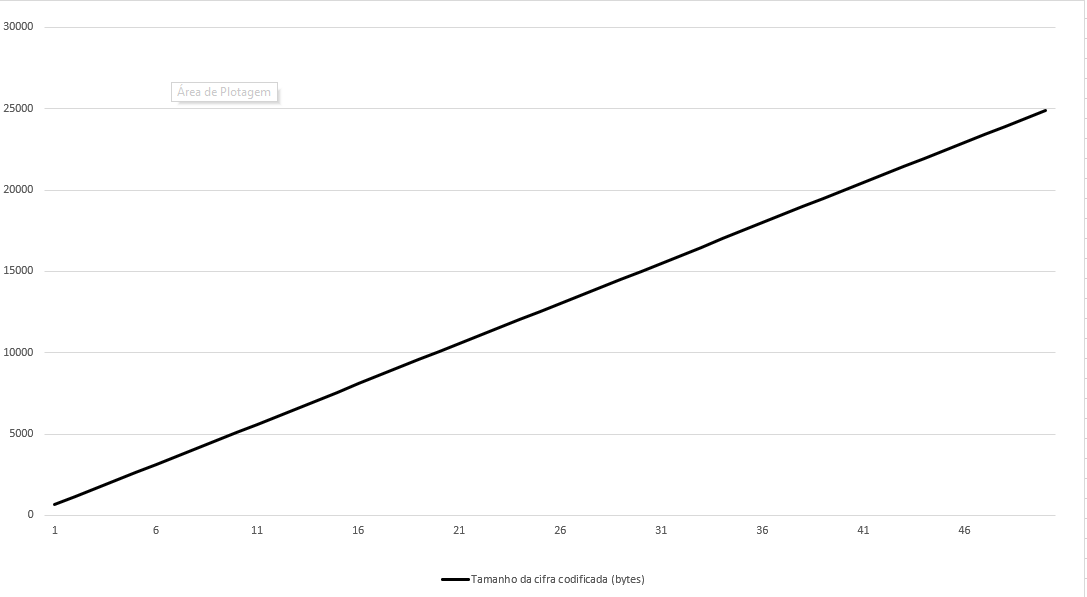
\includegraphics[width=\textwidth]{images/resultados-tamanho-cifra-crescimento.png}
  \caption{Tamanho da cifra ABE em relação à quantidade de atributos utilizados na política de acesso.}
  \label{fig:crescimento-cifra}
\end{figure}

A figura \ref{fig:crescimento-cifra} demonstra o crescimento do tamanho da cifra em função da quantidade de atributos utilizados na política de acesso. Para esta análise, foram executadas múltiplas aplicações ($n=100$) de criptografia ABE a um mesmo arquivo, variando o tamanho da política de acesso de 1 atributo até 100 atributos.
A geração de políticas de acesso para o experimento utilizou uma estratégia recursiva, da seguinte forma:
A geração de uma política de acesso aleatória com $n$ atributos utiliza a seguinte estratégia recursiva:
se a política contém mais de 1 atributo, escolhe-se um operador lógico de forma aleatória.
O operador lógico admite 2 operandos, então o processo é repetido em cada operando respectivamente com tamanho de política de acesso $k$ e $n-k$, onde $k$ é um número aleatório e $1 < k < n$.
Quando $n = 1$, o nó atual representa um atributo e um atributo aleatório é escolhido.
O mesmo experimento foi executado em 3 cenários, um onde apenas o operador AND é usado na construção da política de acesso aleatória, um onde apenas o operador OR e um onde ambos são usados na geração das políticas, representados pelas linhas AZUL, VERMELHA E VERDE, respectivamente.

Os dados apresentados permitem a inferência de uma função linear na forma $y = ax + b$ que descreva o tamanho esperado de uma cifra $Cf$ em função dos $m$ atributos usados na política de acesso:

\begin{equation}
  \begin{aligned}
    Cf(m) & =  3 a \cdot m + b, \textnormal{ onde } a = 495, b = 164 \textnormal{ e } m > 0
  \end{aligned}
\end{equation}

Considerando que o esquema ABE admite tamanhos arbitrários de política de acesso, a função descrita acima não possui um limite superior.
Isso apresenta o problema para a codificação da cifra em uma transação Ethereum, uma vez que existe um limite prático ao tamanho do bloco e consequentemente, ao tamanho da transação, denominado como \emph{Gas Limit}.
O limite de gas impede que a EVM trave na execução de alguma transação e também ajuda a controlar a taxa de adição de novos blocos à Blockchain, podendo subir ou descer de acordo com algumas métricas de uso da rede, como a quantidade de transações passadas, total de taxas pagas em mineração e quantidade de transações aguardando confirmação.
A figura \ref{fig:serie-gasLimit} mostra a série histórica de valores de limite de gas na rede Ethereum, sendo que o valor mais recente dessa série histórica está em 12.474.388 unidades de gas.
O consumo de gas realizado por uma transação tem seu comportamento detalhado nos anexos G e H do Yellow Paper do Ethereum \cite{Wood2017}.

\begin{figure}[!h]
  \centering
  %\includesvg{images/diagrama-DCPABE.svg}
  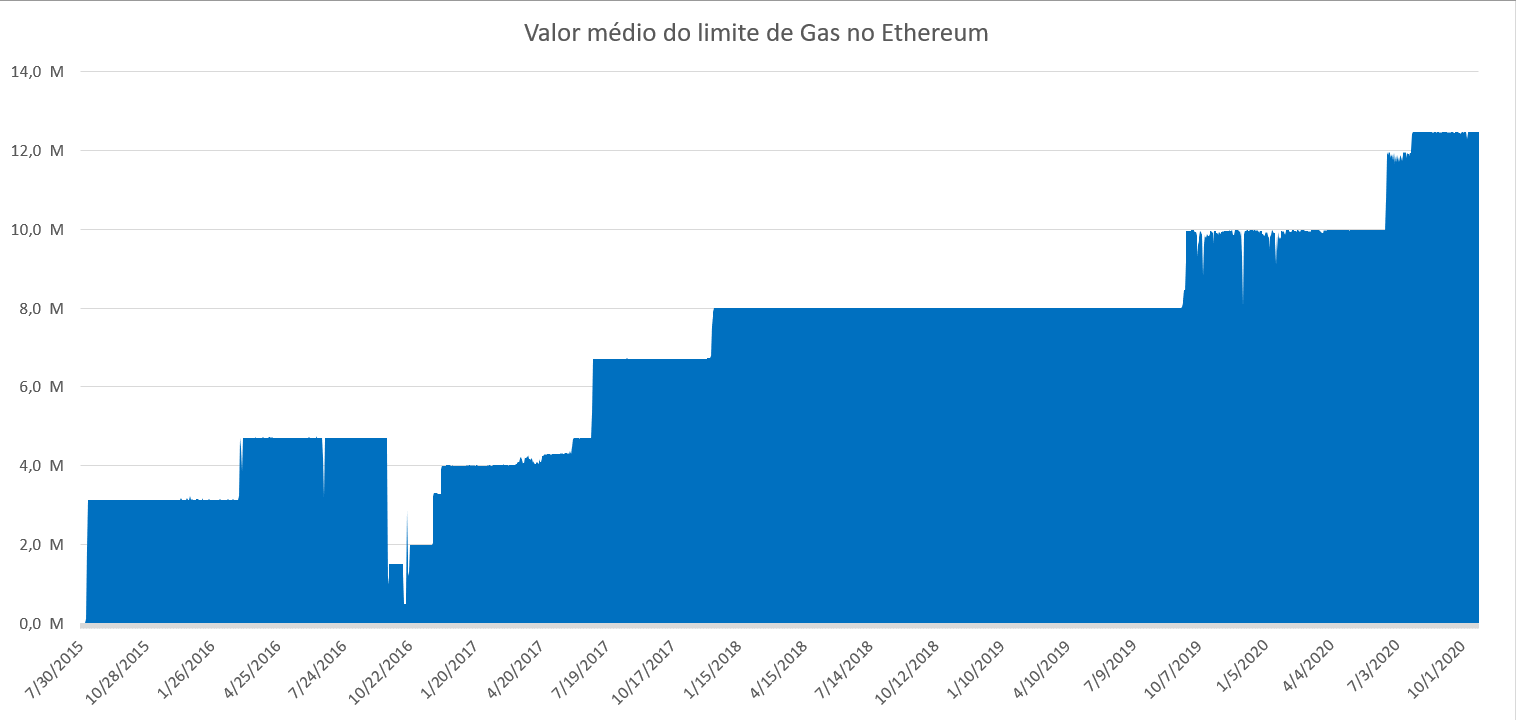
\includegraphics[width=\textwidth]{images/gasLimit.png}
  \caption{Série histórica de valores do limite de gas na rede Ethereum. (Fonte: Etherscan.io)}
  \label{fig:serie-gasLimit}
\end{figure}

O custo em gas de uma transação possui dois componentes, um custo denominado como intrínseco, definido para o caso de uma transação que contenha dados como:

\[g_{0}(n) = G_{transaction} + n \cdot G_{txdatanonzero}\]

E um custo $C$ denominado como geral, definido em detalhes no anexo H do Yellow Paper, basicamente descrito como a soma dos custos de gas das operações executadas em decorrência da transação.
Para uma transação que armazene dados em um Smart Contract, serão cobrados os custos de armazenamento permanente $C_{SSTORE}$, o custo de invocação do contrato $C_{CALL}$ e o custo por byte de alocação de memória temporária, genericamente descrito como possuindo um custo $G_{verylow}$.
O custo de alocação de memória envolve a tarefa de transferência dos dados da transação para a memória durante a execução da função do Smart Contract.
O custo geral estimado para armazenar $n$ bytes de dado seria portanto:

\[C(n) = C_{CALL} + C_{SSTORE} + n \cdot G_{verylow}\]

Portanto, o custo total em gas $g$ de uma transação de armazenamento de $n$ bytes de dados será de:

\begin{equation}
  \begin{aligned}
    g(n) & = g_{0}(n) + C(n)\\
      & = G_{transaction} + n \cdot G_{txdatanonzero} + C_{CALL} + C_{SSTORE} + n \cdot G_{verylow}
  \end{aligned}
\end{equation}

Igualando $g(n)$ ao limite de gas, podemos isolar $n$ e descobrir desta forma qual é o limite do conteúdo que uma transação pode conter:

\begin{equation}
  \begin{aligned}
    gasLimit & = G_{transaction} + n \cdot G_{txdatanonzero} + C_{CALL} + C_{SSTORE} + n \cdot G_{verylow} \\
     n_{max} & = \left\lfloor \frac{gasLimit - (G_{transaction} + C_{CALL} + C_{SSTORE})}{(G_{txdatanonzero} + G_{verylow})} \right\rfloor \\
     n_{max} & = \left\lfloor \frac{12.474.388 - (21000 + 700 + 20000)}{68 + 3} \right\rfloor \\
     n_{max} & = 175.108
  \end{aligned}
\end{equation}

Em um cenário ideal onde não há outras operações sendo realizadas pela função que armazena dados, a transação poderia conter até 175.108 bytes em dados.
No caso de uma cifra ABE, podemos igualar o tamanho da cifra $Cf(m)$ ao valor de $n_{max}$ e deduzir a partir disso a quantidade máxima de atributos $m$ que podem ser usadas em uma política de acesso:

\begin{equation}
  \begin{aligned}
    n_{max} & = 3 \cdot 495 \cdot m + 164 \\
    m_{max} & = \left\lfloor \frac{175.108 - 164}{3 \cdot 495} \right\rfloor \\
    m_{max} & = 117
  \end{aligned}
\end{equation}

Isto significa que, em um cenário ideal de uso onde não há gastos de processamento além do armazenamento da cifra ABE codificada na transação, ainda assim haveria um limite imposto à política de acesso, de forma que sejam utilizado no máximo 177 atributos em sua composição.


%\subsection{Atributos na Blockchain}
%\label{sec:sub:experimento-atributos}

\subsection{Requisições na Blockchain}
\label{sec:sub:experimento-requisicoes}

\subsection{Custos de transação no Ethereum}
\label{sec:sub:experimento-custos}

% -------------------------------------------------------------------- %
\newpage
\section{Conclusões e Trabalhos futuros}

\bibliography{doc}
\bibliographystyle{plainnat}

% -------------------------------------------------------------------- %
\appendix
\section{Taxonomia de profissões na área da saúde}
\label{app:taxonomiaProfissões}

\import{./}{taxonomia-profissões-completo.tex}

\newpage
\section{Projetos de Criptomoedas com suporte nativo à execução de Smart Contracts}
\label{app:outrasCriptomoedasSmartContracts}

\newpage
\section{Código fonte dos Smart Contracts}
\label{app:codigoSmartContracts}

\end{document}
